\documentclass[twoside]{book}

% Packages required by doxygen
\usepackage{fixltx2e}
\usepackage{calc}
\usepackage{doxygen}
\usepackage[export]{adjustbox} % also loads graphicx
\usepackage{graphicx}
\usepackage[utf8]{inputenc}
\usepackage{makeidx}
\usepackage{multicol}
\usepackage{multirow}
\PassOptionsToPackage{warn}{textcomp}
\usepackage{textcomp}
\usepackage[nointegrals]{wasysym}
\usepackage[table]{xcolor}

% Font selection
\usepackage[T1]{fontenc}
\usepackage[scaled=.90]{helvet}
\usepackage{courier}
\usepackage{amssymb}
\usepackage{sectsty}
\renewcommand{\familydefault}{\sfdefault}
\allsectionsfont{%
  \fontseries{bc}\selectfont%
  \color{darkgray}%
}
\renewcommand{\DoxyLabelFont}{%
  \fontseries{bc}\selectfont%
  \color{darkgray}%
}
\newcommand{\+}{\discretionary{\mbox{\scriptsize$\hookleftarrow$}}{}{}}

% Page & text layout
\usepackage{geometry}
\geometry{%
  a4paper,%
  top=2.5cm,%
  bottom=2.5cm,%
  left=2.5cm,%
  right=2.5cm%
}
\tolerance=750
\hfuzz=15pt
\hbadness=750
\setlength{\emergencystretch}{15pt}
\setlength{\parindent}{0cm}
\setlength{\parskip}{0.2cm}
\makeatletter
\renewcommand{\paragraph}{%
  \@startsection{paragraph}{4}{0ex}{-1.0ex}{1.0ex}{%
    \normalfont\normalsize\bfseries\SS@parafont%
  }%
}
\renewcommand{\subparagraph}{%
  \@startsection{subparagraph}{5}{0ex}{-1.0ex}{1.0ex}{%
    \normalfont\normalsize\bfseries\SS@subparafont%
  }%
}
\makeatother

% Headers & footers
\usepackage{fancyhdr}
\pagestyle{fancyplain}
\fancyhead[LE]{\fancyplain{}{\bfseries\thepage}}
\fancyhead[CE]{\fancyplain{}{}}
\fancyhead[RE]{\fancyplain{}{\bfseries\leftmark}}
\fancyhead[LO]{\fancyplain{}{\bfseries\rightmark}}
\fancyhead[CO]{\fancyplain{}{}}
\fancyhead[RO]{\fancyplain{}{\bfseries\thepage}}
\fancyfoot[LE]{\fancyplain{}{}}
\fancyfoot[CE]{\fancyplain{}{}}
\fancyfoot[RE]{\fancyplain{}{\bfseries\scriptsize Generated on Tue Feb 10 2015 00\+:13\+:53 for Gaussian E\+S\+I Automated Creator by Doxygen }}
\fancyfoot[LO]{\fancyplain{}{\bfseries\scriptsize Generated on Tue Feb 10 2015 00\+:13\+:53 for Gaussian E\+S\+I Automated Creator by Doxygen }}
\fancyfoot[CO]{\fancyplain{}{}}
\fancyfoot[RO]{\fancyplain{}{}}
\renewcommand{\footrulewidth}{0.4pt}
\renewcommand{\chaptermark}[1]{%
  \markboth{#1}{}%
}
\renewcommand{\sectionmark}[1]{%
  \markright{\thesection\ #1}%
}

% Indices & bibliography
\usepackage{natbib}
\usepackage[titles]{tocloft}
\setcounter{tocdepth}{3}
\setcounter{secnumdepth}{5}
\makeindex

% Hyperlinks (required, but should be loaded last)
\usepackage{ifpdf}
\ifpdf
  \usepackage[pdftex,pagebackref=true]{hyperref}
\else
  \usepackage[ps2pdf,pagebackref=true]{hyperref}
\fi
\hypersetup{%
  colorlinks=true,%
  linkcolor=blue,%
  citecolor=blue,%
  unicode%
}

% Custom commands
\newcommand{\clearemptydoublepage}{%
  \newpage{\pagestyle{empty}\cleardoublepage}%
}


%===== C O N T E N T S =====

\begin{document}

% Titlepage & ToC
\hypersetup{pageanchor=false,
             bookmarks=true,
             bookmarksnumbered=true,
             pdfencoding=unicode
            }
\pagenumbering{roman}
\begin{titlepage}
\vspace*{7cm}
\begin{center}%
{\Large Gaussian E\+S\+I Automated Creator }\\
\vspace*{1cm}
{\large Generated by Doxygen 1.8.9.1}\\
\vspace*{0.5cm}
{\small Tue Feb 10 2015 00:13:53}\\
\end{center}
\end{titlepage}
\clearemptydoublepage
\tableofcontents
\clearemptydoublepage
\pagenumbering{arabic}
\hypersetup{pageanchor=true}

%--- Begin generated contents ---
\chapter{Hierarchical Index}
\section{Class Hierarchy}
This inheritance list is sorted roughly, but not completely, alphabetically\+:\begin{DoxyCompactList}
\item \contentsline{section}{Atom}{\pageref{struct_atom}}{}
\item \contentsline{section}{Log\+Parser}{\pageref{class_log_parser}}{}
\item Q\+Abstract\+Table\+Model\begin{DoxyCompactList}
\item \contentsline{section}{File\+Manager}{\pageref{class_file_manager}}{}
\end{DoxyCompactList}
\item Q\+File\begin{DoxyCompactList}
\item \contentsline{section}{Checkable\+File}{\pageref{class_checkable_file}}{}
\end{DoxyCompactList}
\item Q\+File\+Dialog\begin{DoxyCompactList}
\item \contentsline{section}{Check\+File\+Dialog}{\pageref{class_check_file_dialog}}{}
\end{DoxyCompactList}
\item Q\+Main\+Window\begin{DoxyCompactList}
\item \contentsline{section}{Geac}{\pageref{class_geac}}{}
\end{DoxyCompactList}
\item Q\+Object\begin{DoxyCompactList}
\item \contentsline{section}{Esi\+Writer}{\pageref{class_esi_writer}}{}
\end{DoxyCompactList}
\item Q\+Styled\+Item\+Delegate\begin{DoxyCompactList}
\item \contentsline{section}{File\+Manager\+Delegate}{\pageref{class_file_manager_delegate}}{}
\end{DoxyCompactList}
\end{DoxyCompactList}

\chapter{Class Index}
\section{Class List}
Here are the classes, structs, unions and interfaces with brief descriptions\+:\begin{DoxyCompactList}
\item\contentsline{section}{\hyperlink{struct_atom}{Atom} }{\pageref{struct_atom}}{}
\item\contentsline{section}{\hyperlink{class_checkable_file}{Checkable\+File} }{\pageref{class_checkable_file}}{}
\item\contentsline{section}{\hyperlink{class_check_file_dialog}{Check\+File\+Dialog} }{\pageref{class_check_file_dialog}}{}
\item\contentsline{section}{\hyperlink{class_esi_writer}{Esi\+Writer} }{\pageref{class_esi_writer}}{}
\item\contentsline{section}{\hyperlink{class_file_manager}{File\+Manager} }{\pageref{class_file_manager}}{}
\item\contentsline{section}{\hyperlink{class_file_manager_delegate}{File\+Manager\+Delegate} }{\pageref{class_file_manager_delegate}}{}
\item\contentsline{section}{\hyperlink{class_geac}{Geac} }{\pageref{class_geac}}{}
\item\contentsline{section}{\hyperlink{class_log_parser}{Log\+Parser} }{\pageref{class_log_parser}}{}
\end{DoxyCompactList}

\chapter{File Index}
\section{File List}
Here is a list of all files with brief descriptions\+:\begin{DoxyCompactList}
\item\contentsline{section}{src/\hyperlink{checkablefile_8cpp}{checkablefile.\+cpp} }{\pageref{checkablefile_8cpp}}{}
\item\contentsline{section}{src/\hyperlink{checkablefile_8h}{checkablefile.\+h} }{\pageref{checkablefile_8h}}{}
\item\contentsline{section}{src/\hyperlink{checkfiledialog_8cpp}{checkfiledialog.\+cpp} }{\pageref{checkfiledialog_8cpp}}{}
\item\contentsline{section}{src/\hyperlink{checkfiledialog_8h}{checkfiledialog.\+h} }{\pageref{checkfiledialog_8h}}{}
\item\contentsline{section}{src/\hyperlink{esiwriter_8cpp}{esiwriter.\+cpp} }{\pageref{esiwriter_8cpp}}{}
\item\contentsline{section}{src/\hyperlink{esiwriter_8h}{esiwriter.\+h} }{\pageref{esiwriter_8h}}{}
\item\contentsline{section}{src/\hyperlink{filemanager_8cpp}{filemanager.\+cpp} }{\pageref{filemanager_8cpp}}{}
\item\contentsline{section}{src/\hyperlink{filemanager_8h}{filemanager.\+h} }{\pageref{filemanager_8h}}{}
\item\contentsline{section}{src/\hyperlink{filemanagerdelegate_8cpp}{filemanagerdelegate.\+cpp} }{\pageref{filemanagerdelegate_8cpp}}{}
\item\contentsline{section}{src/\hyperlink{filemanagerdelegate_8h}{filemanagerdelegate.\+h} }{\pageref{filemanagerdelegate_8h}}{}
\item\contentsline{section}{src/\hyperlink{geac_8cpp}{geac.\+cpp} }{\pageref{geac_8cpp}}{}
\item\contentsline{section}{src/\hyperlink{geac_8h}{geac.\+h} }{\pageref{geac_8h}}{}
\item\contentsline{section}{src/\hyperlink{logparser_8cpp}{logparser.\+cpp} }{\pageref{logparser_8cpp}}{}
\item\contentsline{section}{src/\hyperlink{logparser_8h}{logparser.\+h} }{\pageref{logparser_8h}}{}
\item\contentsline{section}{src/\hyperlink{main_8cpp}{main.\+cpp} }{\pageref{main_8cpp}}{}
\end{DoxyCompactList}

\chapter{Class Documentation}
\hypertarget{struct_atom}{}\section{Atom Struct Reference}
\label{struct_atom}\index{Atom@{Atom}}


{\ttfamily \#include $<$checkablefile.\+h$>$}

\subsection*{Public Attributes}
\begin{DoxyCompactItemize}
\item 
Q\+String \hyperlink{struct_atom_ac3240f6db77b22d77f379a28aad5be1a}{element}
\item 
double \hyperlink{struct_atom_a382da4a2a8d20faa2fd1eca986f44056}{x}
\item 
double \hyperlink{struct_atom_aab210323240ea76e6f866113e590cd22}{y}
\item 
double \hyperlink{struct_atom_af1c8b6cd65e2a489b9be339efd7a77ac}{z}
\end{DoxyCompactItemize}


\subsection{Member Data Documentation}
\hypertarget{struct_atom_ac3240f6db77b22d77f379a28aad5be1a}{}\index{Atom@{Atom}!element@{element}}
\index{element@{element}!Atom@{Atom}}
\subsubsection[{element}]{\setlength{\rightskip}{0pt plus 5cm}Q\+String Atom\+::element}\label{struct_atom_ac3240f6db77b22d77f379a28aad5be1a}
\hypertarget{struct_atom_a382da4a2a8d20faa2fd1eca986f44056}{}\index{Atom@{Atom}!x@{x}}
\index{x@{x}!Atom@{Atom}}
\subsubsection[{x}]{\setlength{\rightskip}{0pt plus 5cm}double Atom\+::x}\label{struct_atom_a382da4a2a8d20faa2fd1eca986f44056}
\hypertarget{struct_atom_aab210323240ea76e6f866113e590cd22}{}\index{Atom@{Atom}!y@{y}}
\index{y@{y}!Atom@{Atom}}
\subsubsection[{y}]{\setlength{\rightskip}{0pt plus 5cm}double Atom\+::y}\label{struct_atom_aab210323240ea76e6f866113e590cd22}
\hypertarget{struct_atom_af1c8b6cd65e2a489b9be339efd7a77ac}{}\index{Atom@{Atom}!z@{z}}
\index{z@{z}!Atom@{Atom}}
\subsubsection[{z}]{\setlength{\rightskip}{0pt plus 5cm}double Atom\+::z}\label{struct_atom_af1c8b6cd65e2a489b9be339efd7a77ac}


The documentation for this struct was generated from the following file\+:\begin{DoxyCompactItemize}
\item 
src/\hyperlink{checkablefile_8h}{checkablefile.\+h}\end{DoxyCompactItemize}

\hypertarget{class_checkable_file}{}\section{Checkable\+File Class Reference}
\label{class_checkable_file}\index{Checkable\+File@{Checkable\+File}}


{\ttfamily \#include $<$checkablefile.\+h$>$}

Inheritance diagram for Checkable\+File\+:\begin{figure}[H]
\begin{center}
\leavevmode
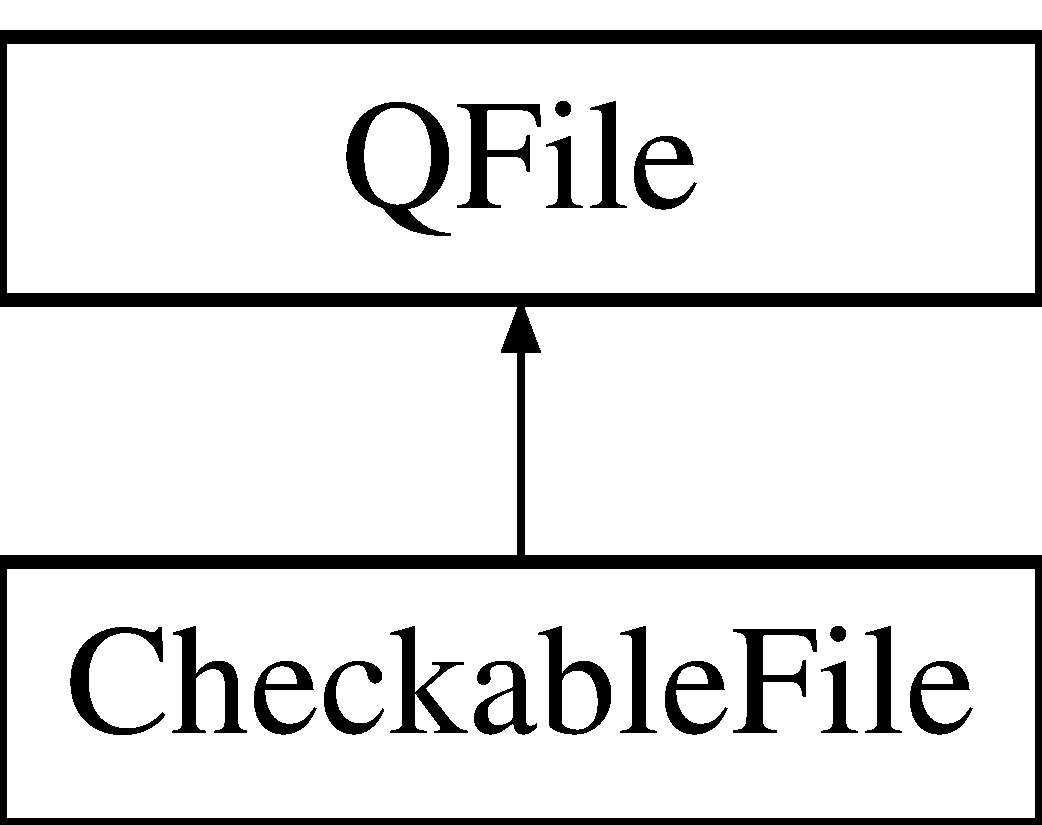
\includegraphics[height=2.000000cm]{class_checkable_file}
\end{center}
\end{figure}
\subsection*{Public Slots}
\begin{DoxyCompactItemize}
\item 
void \hyperlink{class_checkable_file_ac2436dd7ef1249c9cf5c33829b054284}{set\+Conversion\+State} (bool boolean)
\item 
void \hyperlink{class_checkable_file_a7edb6361bcdba016c76be3d9c3906d9e}{set\+Conversion\+Required} (bool boolean)
\end{DoxyCompactItemize}
\subsection*{Public Member Functions}
\begin{DoxyCompactItemize}
\item 
\hyperlink{class_checkable_file_a3d8d14bb50d4d49fb1ab1524bf55d9ad}{Checkable\+File} (Q\+Object $\ast$parent)
\item 
\hyperlink{class_checkable_file_a068da52675987aa9f097deccd04ebd11}{Checkable\+File} (\hyperlink{class_checkable_file}{Checkable\+File} \&file)
\item 
\hyperlink{class_checkable_file_a2c59938768966e97b014fffb360a4a02}{Checkable\+File} ()
\item 
bool \hyperlink{class_checkable_file_a114d896750eb28932939fdf85c50eaf7}{get\+Conversion\+State} ()
\item 
bool \hyperlink{class_checkable_file_a7e96997ce040ddfa1f96208cfbd726a7}{get\+Conversion\+Required} ()
\item 
void \hyperlink{class_checkable_file_ab5f603e8fb4b7bca7b23e731605229c6}{set\+Id} (int i)
\item 
int \hyperlink{class_checkable_file_aff4949da0fe81acb339b6160ed0fb694}{get\+Id} ()
\item 
Q\+String \hyperlink{class_checkable_file_a0ef90a49e1d9aac4988fd698b110207e}{display\+Name} ()
\item 
Q\+String \hyperlink{class_checkable_file_ab47013f328c9a8c1d2c69fd0154bf09d}{get\+N\+Atoms} () const 
\item 
void \hyperlink{class_checkable_file_a5b9a73cf9e7c46ff6ad04c471789846d}{set\+N\+Atoms} (const Q\+String \&value)
\item 
Q\+String \hyperlink{class_checkable_file_a6cdf454d74017f9952f2b6a3cf59aa6d}{get\+Hartree\+Fock\+Energy} () const 
\item 
void \hyperlink{class_checkable_file_ad6488c057deefef8773674bb597c87bd}{set\+Hartree\+Fock\+Energy} (const Q\+String \&value)
\item 
Q\+String\+List \hyperlink{class_checkable_file_a19379105e20add41c24030560c5796a5}{get\+Thermochemistry} () const 
\item 
void \hyperlink{class_checkable_file_a454fe6f9bea36029e128983ab13b4a84}{set\+Thermochemistry} (const Q\+String\+List \&value)
\item 
Q\+String\+List \hyperlink{class_checkable_file_a128db7443c7d5e5e9269ecc6086b39aa}{get\+Harmonic\+Frequencies} () const 
\item 
void \hyperlink{class_checkable_file_abe6fbd9aa2e2d632ec4ceb17de91183a}{set\+Harmonic\+Frequencies} (const Q\+String\+List \&value)
\item 
bool \hyperlink{class_checkable_file_ab016dfc40508bbe078034bb6ffda5a1b}{get\+Data\+Extracted} () const 
\item 
void \hyperlink{class_checkable_file_a66cd4a3381d8a3d7520ffadfca00a1c8}{set\+Data\+Extracted} (bool value)
\item 
Q\+List$<$ \hyperlink{struct_atom}{Atom} $>$ \hyperlink{class_checkable_file_abaee99a31f1e823d0d46cee5a8df0d81}{get\+Coordinates} () const 
\item 
void \hyperlink{class_checkable_file_a424b7a32bb6401ead319d8cb38231184}{set\+Coordinates} (const Q\+List$<$ \hyperlink{struct_atom}{Atom} $>$ \&value)
\end{DoxyCompactItemize}


\subsection{Constructor \& Destructor Documentation}
\hypertarget{class_checkable_file_a3d8d14bb50d4d49fb1ab1524bf55d9ad}{}\index{Checkable\+File@{Checkable\+File}!Checkable\+File@{Checkable\+File}}
\index{Checkable\+File@{Checkable\+File}!Checkable\+File@{Checkable\+File}}
\subsubsection[{Checkable\+File}]{\setlength{\rightskip}{0pt plus 5cm}Checkable\+File\+::\+Checkable\+File (
\begin{DoxyParamCaption}
\item[{Q\+Object $\ast$}]{parent}
\end{DoxyParamCaption}
)\hspace{0.3cm}{\ttfamily [explicit]}}\label{class_checkable_file_a3d8d14bb50d4d49fb1ab1524bf55d9ad}
\hypertarget{class_checkable_file_a068da52675987aa9f097deccd04ebd11}{}\index{Checkable\+File@{Checkable\+File}!Checkable\+File@{Checkable\+File}}
\index{Checkable\+File@{Checkable\+File}!Checkable\+File@{Checkable\+File}}
\subsubsection[{Checkable\+File}]{\setlength{\rightskip}{0pt plus 5cm}Checkable\+File\+::\+Checkable\+File (
\begin{DoxyParamCaption}
\item[{{\bf Checkable\+File} \&}]{file}
\end{DoxyParamCaption}
)}\label{class_checkable_file_a068da52675987aa9f097deccd04ebd11}
\hypertarget{class_checkable_file_a2c59938768966e97b014fffb360a4a02}{}\index{Checkable\+File@{Checkable\+File}!Checkable\+File@{Checkable\+File}}
\index{Checkable\+File@{Checkable\+File}!Checkable\+File@{Checkable\+File}}
\subsubsection[{Checkable\+File}]{\setlength{\rightskip}{0pt plus 5cm}Checkable\+File\+::\+Checkable\+File (
\begin{DoxyParamCaption}
{}
\end{DoxyParamCaption}
)}\label{class_checkable_file_a2c59938768966e97b014fffb360a4a02}


\subsection{Member Function Documentation}
\hypertarget{class_checkable_file_a0ef90a49e1d9aac4988fd698b110207e}{}\index{Checkable\+File@{Checkable\+File}!display\+Name@{display\+Name}}
\index{display\+Name@{display\+Name}!Checkable\+File@{Checkable\+File}}
\subsubsection[{display\+Name}]{\setlength{\rightskip}{0pt plus 5cm}Q\+String Checkable\+File\+::display\+Name (
\begin{DoxyParamCaption}
{}
\end{DoxyParamCaption}
)}\label{class_checkable_file_a0ef90a49e1d9aac4988fd698b110207e}
\hypertarget{class_checkable_file_a7e96997ce040ddfa1f96208cfbd726a7}{}\index{Checkable\+File@{Checkable\+File}!get\+Conversion\+Required@{get\+Conversion\+Required}}
\index{get\+Conversion\+Required@{get\+Conversion\+Required}!Checkable\+File@{Checkable\+File}}
\subsubsection[{get\+Conversion\+Required}]{\setlength{\rightskip}{0pt plus 5cm}bool Checkable\+File\+::get\+Conversion\+Required (
\begin{DoxyParamCaption}
{}
\end{DoxyParamCaption}
)}\label{class_checkable_file_a7e96997ce040ddfa1f96208cfbd726a7}
\hypertarget{class_checkable_file_a114d896750eb28932939fdf85c50eaf7}{}\index{Checkable\+File@{Checkable\+File}!get\+Conversion\+State@{get\+Conversion\+State}}
\index{get\+Conversion\+State@{get\+Conversion\+State}!Checkable\+File@{Checkable\+File}}
\subsubsection[{get\+Conversion\+State}]{\setlength{\rightskip}{0pt plus 5cm}bool Checkable\+File\+::get\+Conversion\+State (
\begin{DoxyParamCaption}
{}
\end{DoxyParamCaption}
)}\label{class_checkable_file_a114d896750eb28932939fdf85c50eaf7}
\hypertarget{class_checkable_file_abaee99a31f1e823d0d46cee5a8df0d81}{}\index{Checkable\+File@{Checkable\+File}!get\+Coordinates@{get\+Coordinates}}
\index{get\+Coordinates@{get\+Coordinates}!Checkable\+File@{Checkable\+File}}
\subsubsection[{get\+Coordinates}]{\setlength{\rightskip}{0pt plus 5cm}Q\+List$<$ {\bf Atom} $>$ Checkable\+File\+::get\+Coordinates (
\begin{DoxyParamCaption}
{}
\end{DoxyParamCaption}
) const}\label{class_checkable_file_abaee99a31f1e823d0d46cee5a8df0d81}
\hypertarget{class_checkable_file_ab016dfc40508bbe078034bb6ffda5a1b}{}\index{Checkable\+File@{Checkable\+File}!get\+Data\+Extracted@{get\+Data\+Extracted}}
\index{get\+Data\+Extracted@{get\+Data\+Extracted}!Checkable\+File@{Checkable\+File}}
\subsubsection[{get\+Data\+Extracted}]{\setlength{\rightskip}{0pt plus 5cm}bool Checkable\+File\+::get\+Data\+Extracted (
\begin{DoxyParamCaption}
{}
\end{DoxyParamCaption}
) const}\label{class_checkable_file_ab016dfc40508bbe078034bb6ffda5a1b}
\hypertarget{class_checkable_file_a128db7443c7d5e5e9269ecc6086b39aa}{}\index{Checkable\+File@{Checkable\+File}!get\+Harmonic\+Frequencies@{get\+Harmonic\+Frequencies}}
\index{get\+Harmonic\+Frequencies@{get\+Harmonic\+Frequencies}!Checkable\+File@{Checkable\+File}}
\subsubsection[{get\+Harmonic\+Frequencies}]{\setlength{\rightskip}{0pt plus 5cm}Q\+String\+List Checkable\+File\+::get\+Harmonic\+Frequencies (
\begin{DoxyParamCaption}
{}
\end{DoxyParamCaption}
) const}\label{class_checkable_file_a128db7443c7d5e5e9269ecc6086b39aa}
\hypertarget{class_checkable_file_a6cdf454d74017f9952f2b6a3cf59aa6d}{}\index{Checkable\+File@{Checkable\+File}!get\+Hartree\+Fock\+Energy@{get\+Hartree\+Fock\+Energy}}
\index{get\+Hartree\+Fock\+Energy@{get\+Hartree\+Fock\+Energy}!Checkable\+File@{Checkable\+File}}
\subsubsection[{get\+Hartree\+Fock\+Energy}]{\setlength{\rightskip}{0pt plus 5cm}Q\+String Checkable\+File\+::get\+Hartree\+Fock\+Energy (
\begin{DoxyParamCaption}
{}
\end{DoxyParamCaption}
) const}\label{class_checkable_file_a6cdf454d74017f9952f2b6a3cf59aa6d}
\hypertarget{class_checkable_file_aff4949da0fe81acb339b6160ed0fb694}{}\index{Checkable\+File@{Checkable\+File}!get\+Id@{get\+Id}}
\index{get\+Id@{get\+Id}!Checkable\+File@{Checkable\+File}}
\subsubsection[{get\+Id}]{\setlength{\rightskip}{0pt plus 5cm}int Checkable\+File\+::get\+Id (
\begin{DoxyParamCaption}
{}
\end{DoxyParamCaption}
)}\label{class_checkable_file_aff4949da0fe81acb339b6160ed0fb694}
\hypertarget{class_checkable_file_ab47013f328c9a8c1d2c69fd0154bf09d}{}\index{Checkable\+File@{Checkable\+File}!get\+N\+Atoms@{get\+N\+Atoms}}
\index{get\+N\+Atoms@{get\+N\+Atoms}!Checkable\+File@{Checkable\+File}}
\subsubsection[{get\+N\+Atoms}]{\setlength{\rightskip}{0pt plus 5cm}Q\+String Checkable\+File\+::get\+N\+Atoms (
\begin{DoxyParamCaption}
{}
\end{DoxyParamCaption}
) const}\label{class_checkable_file_ab47013f328c9a8c1d2c69fd0154bf09d}
\hypertarget{class_checkable_file_a19379105e20add41c24030560c5796a5}{}\index{Checkable\+File@{Checkable\+File}!get\+Thermochemistry@{get\+Thermochemistry}}
\index{get\+Thermochemistry@{get\+Thermochemistry}!Checkable\+File@{Checkable\+File}}
\subsubsection[{get\+Thermochemistry}]{\setlength{\rightskip}{0pt plus 5cm}Q\+String\+List Checkable\+File\+::get\+Thermochemistry (
\begin{DoxyParamCaption}
{}
\end{DoxyParamCaption}
) const}\label{class_checkable_file_a19379105e20add41c24030560c5796a5}
\hypertarget{class_checkable_file_a7edb6361bcdba016c76be3d9c3906d9e}{}\index{Checkable\+File@{Checkable\+File}!set\+Conversion\+Required@{set\+Conversion\+Required}}
\index{set\+Conversion\+Required@{set\+Conversion\+Required}!Checkable\+File@{Checkable\+File}}
\subsubsection[{set\+Conversion\+Required}]{\setlength{\rightskip}{0pt plus 5cm}void Checkable\+File\+::set\+Conversion\+Required (
\begin{DoxyParamCaption}
\item[{bool}]{boolean}
\end{DoxyParamCaption}
)\hspace{0.3cm}{\ttfamily [slot]}}\label{class_checkable_file_a7edb6361bcdba016c76be3d9c3906d9e}
\hypertarget{class_checkable_file_ac2436dd7ef1249c9cf5c33829b054284}{}\index{Checkable\+File@{Checkable\+File}!set\+Conversion\+State@{set\+Conversion\+State}}
\index{set\+Conversion\+State@{set\+Conversion\+State}!Checkable\+File@{Checkable\+File}}
\subsubsection[{set\+Conversion\+State}]{\setlength{\rightskip}{0pt plus 5cm}void Checkable\+File\+::set\+Conversion\+State (
\begin{DoxyParamCaption}
\item[{bool}]{boolean}
\end{DoxyParamCaption}
)\hspace{0.3cm}{\ttfamily [slot]}}\label{class_checkable_file_ac2436dd7ef1249c9cf5c33829b054284}
\hypertarget{class_checkable_file_a424b7a32bb6401ead319d8cb38231184}{}\index{Checkable\+File@{Checkable\+File}!set\+Coordinates@{set\+Coordinates}}
\index{set\+Coordinates@{set\+Coordinates}!Checkable\+File@{Checkable\+File}}
\subsubsection[{set\+Coordinates}]{\setlength{\rightskip}{0pt plus 5cm}void Checkable\+File\+::set\+Coordinates (
\begin{DoxyParamCaption}
\item[{const Q\+List$<$ {\bf Atom} $>$ \&}]{value}
\end{DoxyParamCaption}
)}\label{class_checkable_file_a424b7a32bb6401ead319d8cb38231184}
\hypertarget{class_checkable_file_a66cd4a3381d8a3d7520ffadfca00a1c8}{}\index{Checkable\+File@{Checkable\+File}!set\+Data\+Extracted@{set\+Data\+Extracted}}
\index{set\+Data\+Extracted@{set\+Data\+Extracted}!Checkable\+File@{Checkable\+File}}
\subsubsection[{set\+Data\+Extracted}]{\setlength{\rightskip}{0pt plus 5cm}void Checkable\+File\+::set\+Data\+Extracted (
\begin{DoxyParamCaption}
\item[{bool}]{value}
\end{DoxyParamCaption}
)}\label{class_checkable_file_a66cd4a3381d8a3d7520ffadfca00a1c8}
\hypertarget{class_checkable_file_abe6fbd9aa2e2d632ec4ceb17de91183a}{}\index{Checkable\+File@{Checkable\+File}!set\+Harmonic\+Frequencies@{set\+Harmonic\+Frequencies}}
\index{set\+Harmonic\+Frequencies@{set\+Harmonic\+Frequencies}!Checkable\+File@{Checkable\+File}}
\subsubsection[{set\+Harmonic\+Frequencies}]{\setlength{\rightskip}{0pt plus 5cm}void Checkable\+File\+::set\+Harmonic\+Frequencies (
\begin{DoxyParamCaption}
\item[{const Q\+String\+List \&}]{value}
\end{DoxyParamCaption}
)}\label{class_checkable_file_abe6fbd9aa2e2d632ec4ceb17de91183a}
\hypertarget{class_checkable_file_ad6488c057deefef8773674bb597c87bd}{}\index{Checkable\+File@{Checkable\+File}!set\+Hartree\+Fock\+Energy@{set\+Hartree\+Fock\+Energy}}
\index{set\+Hartree\+Fock\+Energy@{set\+Hartree\+Fock\+Energy}!Checkable\+File@{Checkable\+File}}
\subsubsection[{set\+Hartree\+Fock\+Energy}]{\setlength{\rightskip}{0pt plus 5cm}void Checkable\+File\+::set\+Hartree\+Fock\+Energy (
\begin{DoxyParamCaption}
\item[{const Q\+String \&}]{value}
\end{DoxyParamCaption}
)}\label{class_checkable_file_ad6488c057deefef8773674bb597c87bd}
\hypertarget{class_checkable_file_ab5f603e8fb4b7bca7b23e731605229c6}{}\index{Checkable\+File@{Checkable\+File}!set\+Id@{set\+Id}}
\index{set\+Id@{set\+Id}!Checkable\+File@{Checkable\+File}}
\subsubsection[{set\+Id}]{\setlength{\rightskip}{0pt plus 5cm}void Checkable\+File\+::set\+Id (
\begin{DoxyParamCaption}
\item[{int}]{i}
\end{DoxyParamCaption}
)}\label{class_checkable_file_ab5f603e8fb4b7bca7b23e731605229c6}
\hypertarget{class_checkable_file_a5b9a73cf9e7c46ff6ad04c471789846d}{}\index{Checkable\+File@{Checkable\+File}!set\+N\+Atoms@{set\+N\+Atoms}}
\index{set\+N\+Atoms@{set\+N\+Atoms}!Checkable\+File@{Checkable\+File}}
\subsubsection[{set\+N\+Atoms}]{\setlength{\rightskip}{0pt plus 5cm}void Checkable\+File\+::set\+N\+Atoms (
\begin{DoxyParamCaption}
\item[{const Q\+String \&}]{value}
\end{DoxyParamCaption}
)}\label{class_checkable_file_a5b9a73cf9e7c46ff6ad04c471789846d}
\hypertarget{class_checkable_file_a454fe6f9bea36029e128983ab13b4a84}{}\index{Checkable\+File@{Checkable\+File}!set\+Thermochemistry@{set\+Thermochemistry}}
\index{set\+Thermochemistry@{set\+Thermochemistry}!Checkable\+File@{Checkable\+File}}
\subsubsection[{set\+Thermochemistry}]{\setlength{\rightskip}{0pt plus 5cm}void Checkable\+File\+::set\+Thermochemistry (
\begin{DoxyParamCaption}
\item[{const Q\+String\+List \&}]{value}
\end{DoxyParamCaption}
)}\label{class_checkable_file_a454fe6f9bea36029e128983ab13b4a84}


The documentation for this class was generated from the following files\+:\begin{DoxyCompactItemize}
\item 
src/\hyperlink{checkablefile_8h}{checkablefile.\+h}\item 
src/\hyperlink{checkablefile_8cpp}{checkablefile.\+cpp}\end{DoxyCompactItemize}

\hypertarget{class_check_file_dialog}{}\section{Check\+File\+Dialog Class Reference}
\label{class_check_file_dialog}\index{Check\+File\+Dialog@{Check\+File\+Dialog}}


{\ttfamily \#include $<$checkfiledialog.\+h$>$}

Inheritance diagram for Check\+File\+Dialog\+:\begin{figure}[H]
\begin{center}
\leavevmode
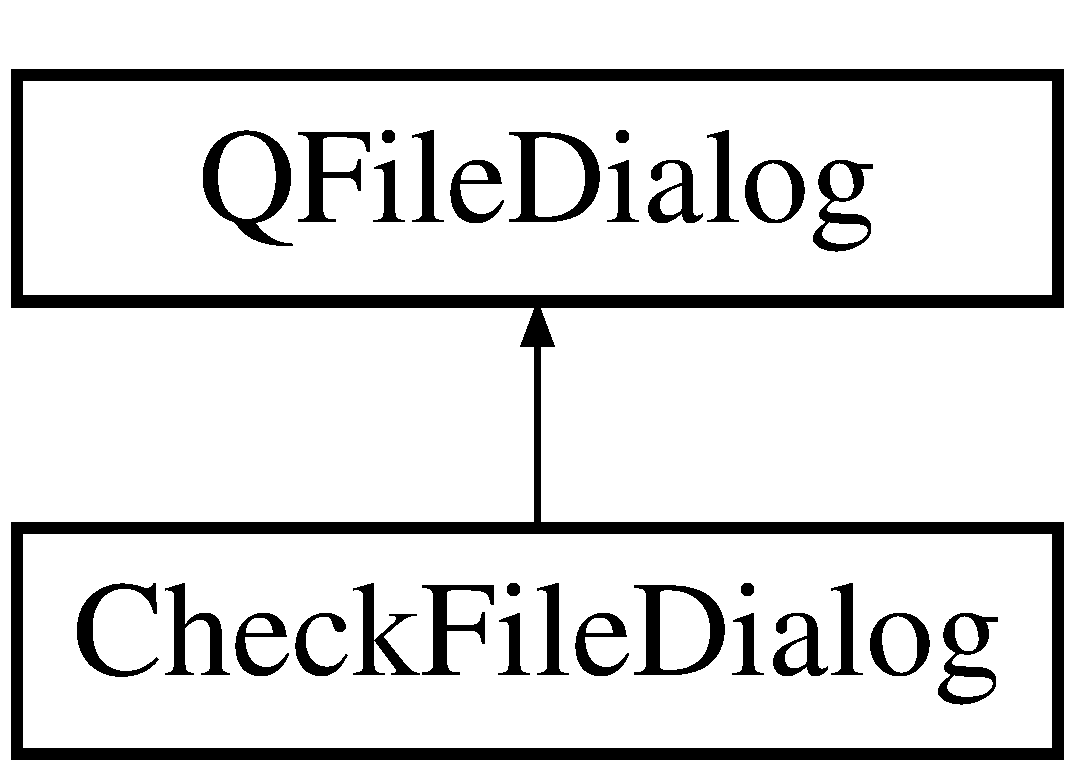
\includegraphics[height=2.000000cm]{class_check_file_dialog}
\end{center}
\end{figure}
\subsection*{Public Types}
\begin{DoxyCompactItemize}
\item 
enum \hyperlink{class_check_file_dialog_aef425279166ddf0cec2e153d80893e80}{file\+Filter} \{ \hyperlink{class_check_file_dialog_aef425279166ddf0cec2e153d80893e80a422bcf31fdb409430f93a05d2384321e}{all}, 
\hyperlink{class_check_file_dialog_aef425279166ddf0cec2e153d80893e80a89aef0892b65192e684d3ea6a6e824f4}{out\+And\+Log}, 
\hyperlink{class_check_file_dialog_aef425279166ddf0cec2e153d80893e80ac75e4d0b89211bb2effd4e1c87275247}{out}, 
\hyperlink{class_check_file_dialog_aef425279166ddf0cec2e153d80893e80a875d4434eae42b0410509ba327d3933e}{log}
 \}
\end{DoxyCompactItemize}
\subsection*{Public Member Functions}
\begin{DoxyCompactItemize}
\item 
\hyperlink{class_check_file_dialog_a85e17297502cb15ef71df1cf747f6454}{Check\+File\+Dialog} ()
\item 
void \hyperlink{class_check_file_dialog_a658bf64019f6bb361e5e5d043e457c4a}{set\+Multiple\+Files\+Mode} ()
\item 
void \hyperlink{class_check_file_dialog_a4e32af3b8b068ec4e5b8f8005239e90b}{set\+Directory\+Mode} ()
\item 
bool \hyperlink{class_check_file_dialog_a8129e12b60b491d22467e50258af4e38}{get\+Recursivity} ()
\item 
int \hyperlink{class_check_file_dialog_aae56141a35759268fe0143386d3258d9}{get\+File\+Filter} ()
\end{DoxyCompactItemize}


\subsection{Member Enumeration Documentation}
\hypertarget{class_check_file_dialog_aef425279166ddf0cec2e153d80893e80}{}\index{Check\+File\+Dialog@{Check\+File\+Dialog}!file\+Filter@{file\+Filter}}
\index{file\+Filter@{file\+Filter}!Check\+File\+Dialog@{Check\+File\+Dialog}}
\subsubsection[{file\+Filter}]{\setlength{\rightskip}{0pt plus 5cm}enum {\bf Check\+File\+Dialog\+::file\+Filter}}\label{class_check_file_dialog_aef425279166ddf0cec2e153d80893e80}
\begin{Desc}
\item[Enumerator]\par
\begin{description}
\index{all@{all}!Check\+File\+Dialog@{Check\+File\+Dialog}}\index{Check\+File\+Dialog@{Check\+File\+Dialog}!all@{all}}\item[{\em 
\hypertarget{class_check_file_dialog_aef425279166ddf0cec2e153d80893e80a422bcf31fdb409430f93a05d2384321e}{}all\label{class_check_file_dialog_aef425279166ddf0cec2e153d80893e80a422bcf31fdb409430f93a05d2384321e}
}]\index{out\+And\+Log@{out\+And\+Log}!Check\+File\+Dialog@{Check\+File\+Dialog}}\index{Check\+File\+Dialog@{Check\+File\+Dialog}!out\+And\+Log@{out\+And\+Log}}\item[{\em 
\hypertarget{class_check_file_dialog_aef425279166ddf0cec2e153d80893e80a89aef0892b65192e684d3ea6a6e824f4}{}out\+And\+Log\label{class_check_file_dialog_aef425279166ddf0cec2e153d80893e80a89aef0892b65192e684d3ea6a6e824f4}
}]\index{out@{out}!Check\+File\+Dialog@{Check\+File\+Dialog}}\index{Check\+File\+Dialog@{Check\+File\+Dialog}!out@{out}}\item[{\em 
\hypertarget{class_check_file_dialog_aef425279166ddf0cec2e153d80893e80ac75e4d0b89211bb2effd4e1c87275247}{}out\label{class_check_file_dialog_aef425279166ddf0cec2e153d80893e80ac75e4d0b89211bb2effd4e1c87275247}
}]\index{log@{log}!Check\+File\+Dialog@{Check\+File\+Dialog}}\index{Check\+File\+Dialog@{Check\+File\+Dialog}!log@{log}}\item[{\em 
\hypertarget{class_check_file_dialog_aef425279166ddf0cec2e153d80893e80a875d4434eae42b0410509ba327d3933e}{}log\label{class_check_file_dialog_aef425279166ddf0cec2e153d80893e80a875d4434eae42b0410509ba327d3933e}
}]\end{description}
\end{Desc}


\subsection{Constructor \& Destructor Documentation}
\hypertarget{class_check_file_dialog_a85e17297502cb15ef71df1cf747f6454}{}\index{Check\+File\+Dialog@{Check\+File\+Dialog}!Check\+File\+Dialog@{Check\+File\+Dialog}}
\index{Check\+File\+Dialog@{Check\+File\+Dialog}!Check\+File\+Dialog@{Check\+File\+Dialog}}
\subsubsection[{Check\+File\+Dialog}]{\setlength{\rightskip}{0pt plus 5cm}Check\+File\+Dialog\+::\+Check\+File\+Dialog (
\begin{DoxyParamCaption}
{}
\end{DoxyParamCaption}
)}\label{class_check_file_dialog_a85e17297502cb15ef71df1cf747f6454}


\subsection{Member Function Documentation}
\hypertarget{class_check_file_dialog_aae56141a35759268fe0143386d3258d9}{}\index{Check\+File\+Dialog@{Check\+File\+Dialog}!get\+File\+Filter@{get\+File\+Filter}}
\index{get\+File\+Filter@{get\+File\+Filter}!Check\+File\+Dialog@{Check\+File\+Dialog}}
\subsubsection[{get\+File\+Filter}]{\setlength{\rightskip}{0pt plus 5cm}int Check\+File\+Dialog\+::get\+File\+Filter (
\begin{DoxyParamCaption}
{}
\end{DoxyParamCaption}
)}\label{class_check_file_dialog_aae56141a35759268fe0143386d3258d9}
\hypertarget{class_check_file_dialog_a8129e12b60b491d22467e50258af4e38}{}\index{Check\+File\+Dialog@{Check\+File\+Dialog}!get\+Recursivity@{get\+Recursivity}}
\index{get\+Recursivity@{get\+Recursivity}!Check\+File\+Dialog@{Check\+File\+Dialog}}
\subsubsection[{get\+Recursivity}]{\setlength{\rightskip}{0pt plus 5cm}bool Check\+File\+Dialog\+::get\+Recursivity (
\begin{DoxyParamCaption}
{}
\end{DoxyParamCaption}
)}\label{class_check_file_dialog_a8129e12b60b491d22467e50258af4e38}
\hypertarget{class_check_file_dialog_a4e32af3b8b068ec4e5b8f8005239e90b}{}\index{Check\+File\+Dialog@{Check\+File\+Dialog}!set\+Directory\+Mode@{set\+Directory\+Mode}}
\index{set\+Directory\+Mode@{set\+Directory\+Mode}!Check\+File\+Dialog@{Check\+File\+Dialog}}
\subsubsection[{set\+Directory\+Mode}]{\setlength{\rightskip}{0pt plus 5cm}void Check\+File\+Dialog\+::set\+Directory\+Mode (
\begin{DoxyParamCaption}
{}
\end{DoxyParamCaption}
)}\label{class_check_file_dialog_a4e32af3b8b068ec4e5b8f8005239e90b}
\hypertarget{class_check_file_dialog_a658bf64019f6bb361e5e5d043e457c4a}{}\index{Check\+File\+Dialog@{Check\+File\+Dialog}!set\+Multiple\+Files\+Mode@{set\+Multiple\+Files\+Mode}}
\index{set\+Multiple\+Files\+Mode@{set\+Multiple\+Files\+Mode}!Check\+File\+Dialog@{Check\+File\+Dialog}}
\subsubsection[{set\+Multiple\+Files\+Mode}]{\setlength{\rightskip}{0pt plus 5cm}void Check\+File\+Dialog\+::set\+Multiple\+Files\+Mode (
\begin{DoxyParamCaption}
{}
\end{DoxyParamCaption}
)}\label{class_check_file_dialog_a658bf64019f6bb361e5e5d043e457c4a}


The documentation for this class was generated from the following files\+:\begin{DoxyCompactItemize}
\item 
src/\hyperlink{checkfiledialog_8h}{checkfiledialog.\+h}\item 
src/\hyperlink{checkfiledialog_8cpp}{checkfiledialog.\+cpp}\end{DoxyCompactItemize}

\hypertarget{class_esi_writer}{}\section{Esi\+Writer Class Reference}
\label{class_esi_writer}\index{Esi\+Writer@{Esi\+Writer}}


{\ttfamily \#include $<$esiwriter.\+h$>$}



Inheritance diagram for Esi\+Writer\+:
\nopagebreak
\begin{figure}[H]
\begin{center}
\leavevmode
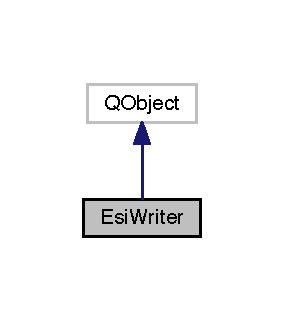
\includegraphics[width=136pt]{class_esi_writer__inherit__graph}
\end{center}
\end{figure}


Collaboration diagram for Esi\+Writer\+:
\nopagebreak
\begin{figure}[H]
\begin{center}
\leavevmode
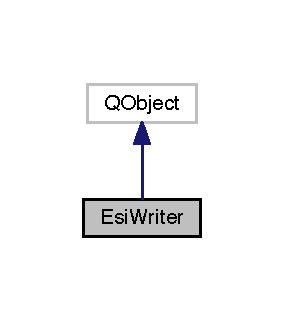
\includegraphics[width=136pt]{class_esi_writer__coll__graph}
\end{center}
\end{figure}
\subsection*{Signals}
\begin{DoxyCompactItemize}
\item 
void \hyperlink{class_esi_writer_a5761a75e40cdd764e9f6f4384db9691f}{file\+Processed} ()
\end{DoxyCompactItemize}
\subsection*{Public Member Functions}
\begin{DoxyCompactItemize}
\item 
\hyperlink{class_esi_writer_a4778aeaa6975d47db1af27c803329756}{Esi\+Writer} ()
\item 
\hyperlink{class_esi_writer_a8828e280684c454cb2ffb18355300b29}{Esi\+Writer} (\hyperlink{class_checkable_file}{Checkable\+File} \&input\+File)
\item 
void \hyperlink{class_esi_writer_a74756630da3cb105db6a9804d96544d8}{set\+Input\+File} (\hyperlink{class_checkable_file}{Checkable\+File} \&input\+File)
\item 
void \hyperlink{class_esi_writer_a4fff58c132284f4ace93f1db36d683e0}{set\+Output\+Folder} (Q\+Dir \&output\+Folder)
\item 
void \hyperlink{class_esi_writer_a0dcece5d6d4c3a172b16b053772fd4aa}{set\+Required\+Fields} (bool \&thermochemistry, bool \&harmonic\+Frequencies, bool \&standard\+Coordinates, bool \&hartree\+Fock\+Energy)
\item 
void \hyperlink{class_esi_writer_a5d9ec4ef42a6e0cc41ded636e70b5325}{create\+Esi} ()
\item 
void \hyperlink{class_esi_writer_a1e587bc3832358745e93cbd7206cff5a}{set\+Extension} (Q\+String extension)
\item 
void \hyperlink{class_esi_writer_a641bf40892ae0e06fd9d0a4d5560cc42}{setup\+Extractor} (bool \&thermochemistry, bool \&harmonic\+Frequencies, bool \&standard\+Coordinates, bool \&hartree\+Fock\+Energy, Q\+Dir \&output\+Folder, Q\+String extension)
\end{DoxyCompactItemize}


\subsection{Constructor \& Destructor Documentation}
\hypertarget{class_esi_writer_a4778aeaa6975d47db1af27c803329756}{}\index{Esi\+Writer@{Esi\+Writer}!Esi\+Writer@{Esi\+Writer}}
\index{Esi\+Writer@{Esi\+Writer}!Esi\+Writer@{Esi\+Writer}}
\subsubsection[{Esi\+Writer}]{\setlength{\rightskip}{0pt plus 5cm}Esi\+Writer\+::\+Esi\+Writer (
\begin{DoxyParamCaption}
{}
\end{DoxyParamCaption}
)}\label{class_esi_writer_a4778aeaa6975d47db1af27c803329756}
\hypertarget{class_esi_writer_a8828e280684c454cb2ffb18355300b29}{}\index{Esi\+Writer@{Esi\+Writer}!Esi\+Writer@{Esi\+Writer}}
\index{Esi\+Writer@{Esi\+Writer}!Esi\+Writer@{Esi\+Writer}}
\subsubsection[{Esi\+Writer}]{\setlength{\rightskip}{0pt plus 5cm}Esi\+Writer\+::\+Esi\+Writer (
\begin{DoxyParamCaption}
\item[{{\bf Checkable\+File} \&}]{input\+File}
\end{DoxyParamCaption}
)}\label{class_esi_writer_a8828e280684c454cb2ffb18355300b29}


\subsection{Member Function Documentation}
\hypertarget{class_esi_writer_a5d9ec4ef42a6e0cc41ded636e70b5325}{}\index{Esi\+Writer@{Esi\+Writer}!create\+Esi@{create\+Esi}}
\index{create\+Esi@{create\+Esi}!Esi\+Writer@{Esi\+Writer}}
\subsubsection[{create\+Esi}]{\setlength{\rightskip}{0pt plus 5cm}void Esi\+Writer\+::create\+Esi (
\begin{DoxyParamCaption}
{}
\end{DoxyParamCaption}
)}\label{class_esi_writer_a5d9ec4ef42a6e0cc41ded636e70b5325}
\hypertarget{class_esi_writer_a5761a75e40cdd764e9f6f4384db9691f}{}\index{Esi\+Writer@{Esi\+Writer}!file\+Processed@{file\+Processed}}
\index{file\+Processed@{file\+Processed}!Esi\+Writer@{Esi\+Writer}}
\subsubsection[{file\+Processed}]{\setlength{\rightskip}{0pt plus 5cm}void Esi\+Writer\+::file\+Processed (
\begin{DoxyParamCaption}
{}
\end{DoxyParamCaption}
)\hspace{0.3cm}{\ttfamily [signal]}}\label{class_esi_writer_a5761a75e40cdd764e9f6f4384db9691f}
\hypertarget{class_esi_writer_a1e587bc3832358745e93cbd7206cff5a}{}\index{Esi\+Writer@{Esi\+Writer}!set\+Extension@{set\+Extension}}
\index{set\+Extension@{set\+Extension}!Esi\+Writer@{Esi\+Writer}}
\subsubsection[{set\+Extension}]{\setlength{\rightskip}{0pt plus 5cm}void Esi\+Writer\+::set\+Extension (
\begin{DoxyParamCaption}
\item[{Q\+String}]{extension}
\end{DoxyParamCaption}
)}\label{class_esi_writer_a1e587bc3832358745e93cbd7206cff5a}
\hypertarget{class_esi_writer_a74756630da3cb105db6a9804d96544d8}{}\index{Esi\+Writer@{Esi\+Writer}!set\+Input\+File@{set\+Input\+File}}
\index{set\+Input\+File@{set\+Input\+File}!Esi\+Writer@{Esi\+Writer}}
\subsubsection[{set\+Input\+File}]{\setlength{\rightskip}{0pt plus 5cm}void Esi\+Writer\+::set\+Input\+File (
\begin{DoxyParamCaption}
\item[{{\bf Checkable\+File} \&}]{input\+File}
\end{DoxyParamCaption}
)}\label{class_esi_writer_a74756630da3cb105db6a9804d96544d8}
\hypertarget{class_esi_writer_a4fff58c132284f4ace93f1db36d683e0}{}\index{Esi\+Writer@{Esi\+Writer}!set\+Output\+Folder@{set\+Output\+Folder}}
\index{set\+Output\+Folder@{set\+Output\+Folder}!Esi\+Writer@{Esi\+Writer}}
\subsubsection[{set\+Output\+Folder}]{\setlength{\rightskip}{0pt plus 5cm}void Esi\+Writer\+::set\+Output\+Folder (
\begin{DoxyParamCaption}
\item[{Q\+Dir \&}]{output\+Folder}
\end{DoxyParamCaption}
)}\label{class_esi_writer_a4fff58c132284f4ace93f1db36d683e0}
\hypertarget{class_esi_writer_a0dcece5d6d4c3a172b16b053772fd4aa}{}\index{Esi\+Writer@{Esi\+Writer}!set\+Required\+Fields@{set\+Required\+Fields}}
\index{set\+Required\+Fields@{set\+Required\+Fields}!Esi\+Writer@{Esi\+Writer}}
\subsubsection[{set\+Required\+Fields}]{\setlength{\rightskip}{0pt plus 5cm}void Esi\+Writer\+::set\+Required\+Fields (
\begin{DoxyParamCaption}
\item[{bool \&}]{thermochemistry, }
\item[{bool \&}]{harmonic\+Frequencies, }
\item[{bool \&}]{standard\+Coordinates, }
\item[{bool \&}]{hartree\+Fock\+Energy}
\end{DoxyParamCaption}
)}\label{class_esi_writer_a0dcece5d6d4c3a172b16b053772fd4aa}
\hypertarget{class_esi_writer_a641bf40892ae0e06fd9d0a4d5560cc42}{}\index{Esi\+Writer@{Esi\+Writer}!setup\+Extractor@{setup\+Extractor}}
\index{setup\+Extractor@{setup\+Extractor}!Esi\+Writer@{Esi\+Writer}}
\subsubsection[{setup\+Extractor}]{\setlength{\rightskip}{0pt plus 5cm}void Esi\+Writer\+::setup\+Extractor (
\begin{DoxyParamCaption}
\item[{bool \&}]{thermochemistry, }
\item[{bool \&}]{harmonic\+Frequencies, }
\item[{bool \&}]{standard\+Coordinates, }
\item[{bool \&}]{hartree\+Fock\+Energy, }
\item[{Q\+Dir \&}]{output\+Folder, }
\item[{Q\+String}]{extension}
\end{DoxyParamCaption}
)}\label{class_esi_writer_a641bf40892ae0e06fd9d0a4d5560cc42}


The documentation for this class was generated from the following files\+:\begin{DoxyCompactItemize}
\item 
src/\hyperlink{esiwriter_8h}{esiwriter.\+h}\item 
src/\hyperlink{esiwriter_8cpp}{esiwriter.\+cpp}\end{DoxyCompactItemize}

\hypertarget{class_file_manager}{}\section{File\+Manager Class Reference}
\label{class_file_manager}\index{File\+Manager@{File\+Manager}}


{\ttfamily \#include $<$filemanager.\+h$>$}

Inheritance diagram for File\+Manager\+:\begin{figure}[H]
\begin{center}
\leavevmode
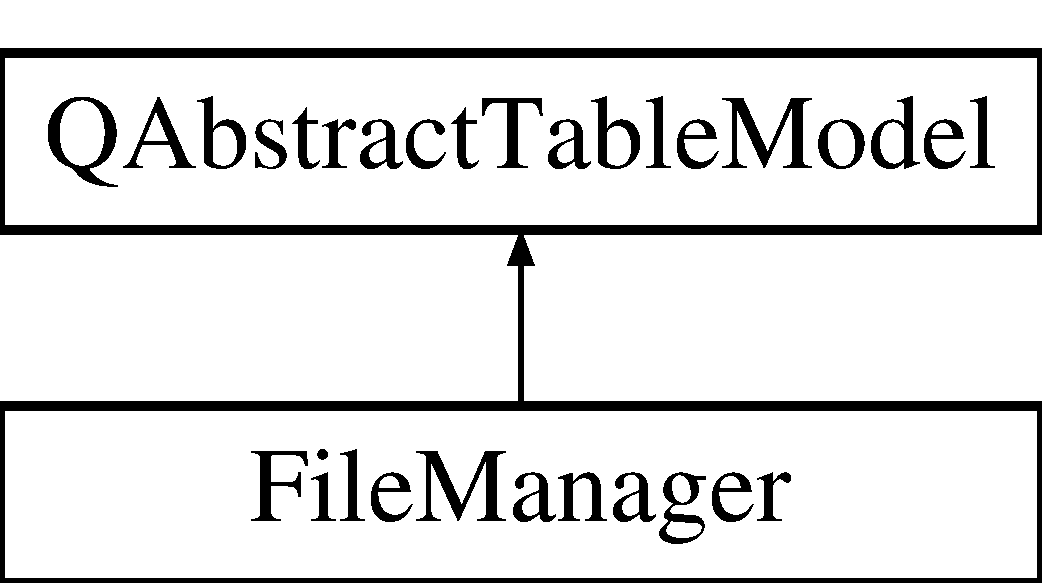
\includegraphics[height=2.000000cm]{class_file_manager}
\end{center}
\end{figure}
\subsection*{Signals}
\begin{DoxyCompactItemize}
\item 
void \hyperlink{class_file_manager_a122e43a43028aaa6e1fafe3a2966cc72}{event\+To\+Display} (Q\+String string)
\end{DoxyCompactItemize}
\subsection*{Public Member Functions}
\begin{DoxyCompactItemize}
\item 
\hyperlink{class_file_manager_aed06615dba6e3987ba4f129505e92edc}{File\+Manager} (Q\+Object $\ast$parent=0)
\item 
int \hyperlink{class_file_manager_aa9d31eb3298e9d05834ab95beb7d2bb5}{row\+Count} (const Q\+Model\+Index \&parent) const 
\item 
int \hyperlink{class_file_manager_a7764e12ab002099b462242ff9bb5337c}{row\+Count} () const 
\item 
int \hyperlink{class_file_manager_ae2423ac9abd3c52d156222cefef3555d}{column\+Count} (const Q\+Model\+Index \&parent) const 
\item 
Q\+Variant \hyperlink{class_file_manager_ab4ad090512825bc604b437be76bc5b46}{data} (const Q\+Model\+Index \&index, int role) const 
\item 
bool \hyperlink{class_file_manager_a5cf1a76c4ab08028ff10468086bdaf92}{set\+Data} (const Q\+Model\+Index \&index, const Q\+Variant \&value, int role)
\item 
Q\+String \hyperlink{class_file_manager_a40338fced75a011297a6cd96da82aa0b}{get\+File\+Path} (int row)
\item 
\hyperlink{class_checkable_file}{Checkable\+File} \& \hyperlink{class_file_manager_a93ffce845f7df82220f3dc450a4fb8fe}{get\+File} (int i)
\item 
\hyperlink{class_checkable_file}{Checkable\+File} $\ast$ \hyperlink{class_file_manager_a3d3c605f92a96d971f18fcdfb283443a}{get\+File\+By\+Id} (int id)
\item 
Q\+Variant \hyperlink{class_file_manager_a158b776ba8de289ce669302ab35367c8}{header\+Data} (int section, Qt\+::\+Orientation orientation, int role) const 
\item 
int \hyperlink{class_file_manager_a4a64b560d32e734dbd42acf6303f9397}{add\+File} (\hyperlink{class_checkable_file}{Checkable\+File} $\ast$file)
\item 
void \hyperlink{class_file_manager_a69455bdd744fdad91a21ca383e93ef7a}{clear\+Files} ()
\item 
bool \hyperlink{class_file_manager_a4505478c3876877d38486994910e35d6}{get\+Required\+Conversion} (Q\+Model\+Index \&index)
\item 
bool \hyperlink{class_file_manager_a38c9259c6681263406ad2c2b21d06aa4}{get\+Required\+Conversion} (int i)
\item 
void \hyperlink{class_file_manager_a354563436fd7d1545edb98c4d9b5de98}{set\+Converted} (int i)
\end{DoxyCompactItemize}


\subsection{Constructor \& Destructor Documentation}
\hypertarget{class_file_manager_aed06615dba6e3987ba4f129505e92edc}{}\index{File\+Manager@{File\+Manager}!File\+Manager@{File\+Manager}}
\index{File\+Manager@{File\+Manager}!File\+Manager@{File\+Manager}}
\subsubsection[{File\+Manager}]{\setlength{\rightskip}{0pt plus 5cm}File\+Manager\+::\+File\+Manager (
\begin{DoxyParamCaption}
\item[{Q\+Object $\ast$}]{parent = {\ttfamily 0}}
\end{DoxyParamCaption}
)}\label{class_file_manager_aed06615dba6e3987ba4f129505e92edc}


\subsection{Member Function Documentation}
\hypertarget{class_file_manager_a4a64b560d32e734dbd42acf6303f9397}{}\index{File\+Manager@{File\+Manager}!add\+File@{add\+File}}
\index{add\+File@{add\+File}!File\+Manager@{File\+Manager}}
\subsubsection[{add\+File}]{\setlength{\rightskip}{0pt plus 5cm}int File\+Manager\+::add\+File (
\begin{DoxyParamCaption}
\item[{{\bf Checkable\+File} $\ast$}]{file}
\end{DoxyParamCaption}
)}\label{class_file_manager_a4a64b560d32e734dbd42acf6303f9397}
\hypertarget{class_file_manager_a69455bdd744fdad91a21ca383e93ef7a}{}\index{File\+Manager@{File\+Manager}!clear\+Files@{clear\+Files}}
\index{clear\+Files@{clear\+Files}!File\+Manager@{File\+Manager}}
\subsubsection[{clear\+Files}]{\setlength{\rightskip}{0pt plus 5cm}void File\+Manager\+::clear\+Files (
\begin{DoxyParamCaption}
{}
\end{DoxyParamCaption}
)}\label{class_file_manager_a69455bdd744fdad91a21ca383e93ef7a}
\hypertarget{class_file_manager_ae2423ac9abd3c52d156222cefef3555d}{}\index{File\+Manager@{File\+Manager}!column\+Count@{column\+Count}}
\index{column\+Count@{column\+Count}!File\+Manager@{File\+Manager}}
\subsubsection[{column\+Count}]{\setlength{\rightskip}{0pt plus 5cm}int File\+Manager\+::column\+Count (
\begin{DoxyParamCaption}
\item[{const Q\+Model\+Index \&}]{parent}
\end{DoxyParamCaption}
) const}\label{class_file_manager_ae2423ac9abd3c52d156222cefef3555d}
\hypertarget{class_file_manager_ab4ad090512825bc604b437be76bc5b46}{}\index{File\+Manager@{File\+Manager}!data@{data}}
\index{data@{data}!File\+Manager@{File\+Manager}}
\subsubsection[{data}]{\setlength{\rightskip}{0pt plus 5cm}Q\+Variant File\+Manager\+::data (
\begin{DoxyParamCaption}
\item[{const Q\+Model\+Index \&}]{index, }
\item[{int}]{role}
\end{DoxyParamCaption}
) const}\label{class_file_manager_ab4ad090512825bc604b437be76bc5b46}
\hypertarget{class_file_manager_a122e43a43028aaa6e1fafe3a2966cc72}{}\index{File\+Manager@{File\+Manager}!event\+To\+Display@{event\+To\+Display}}
\index{event\+To\+Display@{event\+To\+Display}!File\+Manager@{File\+Manager}}
\subsubsection[{event\+To\+Display}]{\setlength{\rightskip}{0pt plus 5cm}void File\+Manager\+::event\+To\+Display (
\begin{DoxyParamCaption}
\item[{Q\+String}]{string}
\end{DoxyParamCaption}
)\hspace{0.3cm}{\ttfamily [signal]}}\label{class_file_manager_a122e43a43028aaa6e1fafe3a2966cc72}
\hypertarget{class_file_manager_a93ffce845f7df82220f3dc450a4fb8fe}{}\index{File\+Manager@{File\+Manager}!get\+File@{get\+File}}
\index{get\+File@{get\+File}!File\+Manager@{File\+Manager}}
\subsubsection[{get\+File}]{\setlength{\rightskip}{0pt plus 5cm}{\bf Checkable\+File} \& File\+Manager\+::get\+File (
\begin{DoxyParamCaption}
\item[{int}]{i}
\end{DoxyParamCaption}
)}\label{class_file_manager_a93ffce845f7df82220f3dc450a4fb8fe}
\hypertarget{class_file_manager_a3d3c605f92a96d971f18fcdfb283443a}{}\index{File\+Manager@{File\+Manager}!get\+File\+By\+Id@{get\+File\+By\+Id}}
\index{get\+File\+By\+Id@{get\+File\+By\+Id}!File\+Manager@{File\+Manager}}
\subsubsection[{get\+File\+By\+Id}]{\setlength{\rightskip}{0pt plus 5cm}{\bf Checkable\+File} $\ast$ File\+Manager\+::get\+File\+By\+Id (
\begin{DoxyParamCaption}
\item[{int}]{id}
\end{DoxyParamCaption}
)}\label{class_file_manager_a3d3c605f92a96d971f18fcdfb283443a}
\hypertarget{class_file_manager_a40338fced75a011297a6cd96da82aa0b}{}\index{File\+Manager@{File\+Manager}!get\+File\+Path@{get\+File\+Path}}
\index{get\+File\+Path@{get\+File\+Path}!File\+Manager@{File\+Manager}}
\subsubsection[{get\+File\+Path}]{\setlength{\rightskip}{0pt plus 5cm}Q\+String File\+Manager\+::get\+File\+Path (
\begin{DoxyParamCaption}
\item[{int}]{row}
\end{DoxyParamCaption}
)}\label{class_file_manager_a40338fced75a011297a6cd96da82aa0b}
\hypertarget{class_file_manager_a4505478c3876877d38486994910e35d6}{}\index{File\+Manager@{File\+Manager}!get\+Required\+Conversion@{get\+Required\+Conversion}}
\index{get\+Required\+Conversion@{get\+Required\+Conversion}!File\+Manager@{File\+Manager}}
\subsubsection[{get\+Required\+Conversion}]{\setlength{\rightskip}{0pt plus 5cm}bool File\+Manager\+::get\+Required\+Conversion (
\begin{DoxyParamCaption}
\item[{Q\+Model\+Index \&}]{index}
\end{DoxyParamCaption}
)}\label{class_file_manager_a4505478c3876877d38486994910e35d6}
\hypertarget{class_file_manager_a38c9259c6681263406ad2c2b21d06aa4}{}\index{File\+Manager@{File\+Manager}!get\+Required\+Conversion@{get\+Required\+Conversion}}
\index{get\+Required\+Conversion@{get\+Required\+Conversion}!File\+Manager@{File\+Manager}}
\subsubsection[{get\+Required\+Conversion}]{\setlength{\rightskip}{0pt plus 5cm}bool File\+Manager\+::get\+Required\+Conversion (
\begin{DoxyParamCaption}
\item[{int}]{i}
\end{DoxyParamCaption}
)}\label{class_file_manager_a38c9259c6681263406ad2c2b21d06aa4}
\hypertarget{class_file_manager_a158b776ba8de289ce669302ab35367c8}{}\index{File\+Manager@{File\+Manager}!header\+Data@{header\+Data}}
\index{header\+Data@{header\+Data}!File\+Manager@{File\+Manager}}
\subsubsection[{header\+Data}]{\setlength{\rightskip}{0pt plus 5cm}Q\+Variant File\+Manager\+::header\+Data (
\begin{DoxyParamCaption}
\item[{int}]{section, }
\item[{Qt\+::\+Orientation}]{orientation, }
\item[{int}]{role}
\end{DoxyParamCaption}
) const}\label{class_file_manager_a158b776ba8de289ce669302ab35367c8}
\hypertarget{class_file_manager_aa9d31eb3298e9d05834ab95beb7d2bb5}{}\index{File\+Manager@{File\+Manager}!row\+Count@{row\+Count}}
\index{row\+Count@{row\+Count}!File\+Manager@{File\+Manager}}
\subsubsection[{row\+Count}]{\setlength{\rightskip}{0pt plus 5cm}int File\+Manager\+::row\+Count (
\begin{DoxyParamCaption}
\item[{const Q\+Model\+Index \&}]{parent}
\end{DoxyParamCaption}
) const}\label{class_file_manager_aa9d31eb3298e9d05834ab95beb7d2bb5}
\hypertarget{class_file_manager_a7764e12ab002099b462242ff9bb5337c}{}\index{File\+Manager@{File\+Manager}!row\+Count@{row\+Count}}
\index{row\+Count@{row\+Count}!File\+Manager@{File\+Manager}}
\subsubsection[{row\+Count}]{\setlength{\rightskip}{0pt plus 5cm}int File\+Manager\+::row\+Count (
\begin{DoxyParamCaption}
{}
\end{DoxyParamCaption}
) const}\label{class_file_manager_a7764e12ab002099b462242ff9bb5337c}
\hypertarget{class_file_manager_a354563436fd7d1545edb98c4d9b5de98}{}\index{File\+Manager@{File\+Manager}!set\+Converted@{set\+Converted}}
\index{set\+Converted@{set\+Converted}!File\+Manager@{File\+Manager}}
\subsubsection[{set\+Converted}]{\setlength{\rightskip}{0pt plus 5cm}void File\+Manager\+::set\+Converted (
\begin{DoxyParamCaption}
\item[{int}]{i}
\end{DoxyParamCaption}
)}\label{class_file_manager_a354563436fd7d1545edb98c4d9b5de98}
\hypertarget{class_file_manager_a5cf1a76c4ab08028ff10468086bdaf92}{}\index{File\+Manager@{File\+Manager}!set\+Data@{set\+Data}}
\index{set\+Data@{set\+Data}!File\+Manager@{File\+Manager}}
\subsubsection[{set\+Data}]{\setlength{\rightskip}{0pt plus 5cm}bool File\+Manager\+::set\+Data (
\begin{DoxyParamCaption}
\item[{const Q\+Model\+Index \&}]{index, }
\item[{const Q\+Variant \&}]{value, }
\item[{int}]{role}
\end{DoxyParamCaption}
)}\label{class_file_manager_a5cf1a76c4ab08028ff10468086bdaf92}


The documentation for this class was generated from the following files\+:\begin{DoxyCompactItemize}
\item 
src/\hyperlink{filemanager_8h}{filemanager.\+h}\item 
src/\hyperlink{filemanager_8cpp}{filemanager.\+cpp}\end{DoxyCompactItemize}

\hypertarget{class_file_manager_delegate}{}\section{File\+Manager\+Delegate Class Reference}
\label{class_file_manager_delegate}\index{File\+Manager\+Delegate@{File\+Manager\+Delegate}}


{\ttfamily \#include $<$filemanagerdelegate.\+h$>$}



Inheritance diagram for File\+Manager\+Delegate\+:
\nopagebreak
\begin{figure}[H]
\begin{center}
\leavevmode
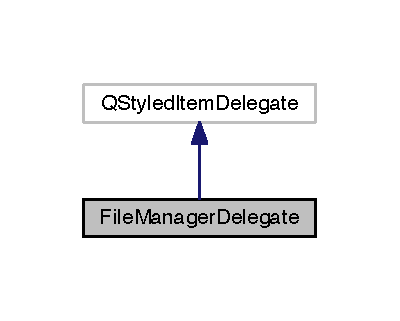
\includegraphics[width=192pt]{class_file_manager_delegate__inherit__graph}
\end{center}
\end{figure}


Collaboration diagram for File\+Manager\+Delegate\+:
\nopagebreak
\begin{figure}[H]
\begin{center}
\leavevmode
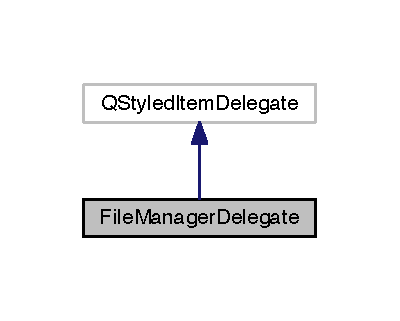
\includegraphics[width=192pt]{class_file_manager_delegate__coll__graph}
\end{center}
\end{figure}
\subsection*{Public Member Functions}
\begin{DoxyCompactItemize}
\item 
\hyperlink{class_file_manager_delegate_a8bae114060c0baa5f455ac3dc8737e38}{File\+Manager\+Delegate} (Q\+Object $\ast$parent=0)
\item 
void \hyperlink{class_file_manager_delegate_aaa74108cf8d09eda076575b9eb029e84}{paint} (Q\+Painter $\ast$painter, const Q\+Style\+Option\+View\+Item \&option, const Q\+Model\+Index \&index) const 
\end{DoxyCompactItemize}


\subsection{Constructor \& Destructor Documentation}
\hypertarget{class_file_manager_delegate_a8bae114060c0baa5f455ac3dc8737e38}{}\index{File\+Manager\+Delegate@{File\+Manager\+Delegate}!File\+Manager\+Delegate@{File\+Manager\+Delegate}}
\index{File\+Manager\+Delegate@{File\+Manager\+Delegate}!File\+Manager\+Delegate@{File\+Manager\+Delegate}}
\subsubsection[{File\+Manager\+Delegate}]{\setlength{\rightskip}{0pt plus 5cm}File\+Manager\+Delegate\+::\+File\+Manager\+Delegate (
\begin{DoxyParamCaption}
\item[{Q\+Object $\ast$}]{parent = {\ttfamily 0}}
\end{DoxyParamCaption}
)\hspace{0.3cm}{\ttfamily [explicit]}}\label{class_file_manager_delegate_a8bae114060c0baa5f455ac3dc8737e38}


\subsection{Member Function Documentation}
\hypertarget{class_file_manager_delegate_aaa74108cf8d09eda076575b9eb029e84}{}\index{File\+Manager\+Delegate@{File\+Manager\+Delegate}!paint@{paint}}
\index{paint@{paint}!File\+Manager\+Delegate@{File\+Manager\+Delegate}}
\subsubsection[{paint}]{\setlength{\rightskip}{0pt plus 5cm}void File\+Manager\+Delegate\+::paint (
\begin{DoxyParamCaption}
\item[{Q\+Painter $\ast$}]{painter, }
\item[{const Q\+Style\+Option\+View\+Item \&}]{option, }
\item[{const Q\+Model\+Index \&}]{index}
\end{DoxyParamCaption}
) const}\label{class_file_manager_delegate_aaa74108cf8d09eda076575b9eb029e84}


The documentation for this class was generated from the following files\+:\begin{DoxyCompactItemize}
\item 
src/\hyperlink{filemanagerdelegate_8h}{filemanagerdelegate.\+h}\item 
src/\hyperlink{filemanagerdelegate_8cpp}{filemanagerdelegate.\+cpp}\end{DoxyCompactItemize}

\hypertarget{class_geac}{}\section{Geac Class Reference}
\label{class_geac}\index{Geac@{Geac}}


{\ttfamily \#include $<$geac.\+h$>$}



Inheritance diagram for Geac\+:
\nopagebreak
\begin{figure}[H]
\begin{center}
\leavevmode
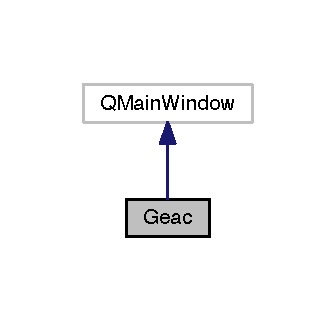
\includegraphics[width=161pt]{class_geac__inherit__graph}
\end{center}
\end{figure}


Collaboration diagram for Geac\+:
\nopagebreak
\begin{figure}[H]
\begin{center}
\leavevmode
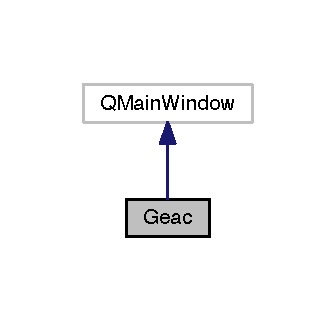
\includegraphics[width=161pt]{class_geac__coll__graph}
\end{center}
\end{figure}
\subsection*{Public Slots}
\begin{DoxyCompactItemize}
\item 
void \hyperlink{class_geac_a088cc7f0bf78e0b741ec63f87cfdfb23}{display\+Log} (Q\+String string)
\item 
void \hyperlink{class_geac_a0f6706f18475db66cc8105ca77ab96ea}{show\+File\+Finished} (int id)
\end{DoxyCompactItemize}
\subsection*{Public Member Functions}
\begin{DoxyCompactItemize}
\item 
\hyperlink{class_geac_a9325c3a5180549943ee201c616a036a3}{Geac} (Q\+Widget $\ast$parent=0)
\end{DoxyCompactItemize}


\subsection{Constructor \& Destructor Documentation}
\hypertarget{class_geac_a9325c3a5180549943ee201c616a036a3}{}\index{Geac@{Geac}!Geac@{Geac}}
\index{Geac@{Geac}!Geac@{Geac}}
\subsubsection[{Geac}]{\setlength{\rightskip}{0pt plus 5cm}Geac\+::\+Geac (
\begin{DoxyParamCaption}
\item[{Q\+Widget $\ast$}]{parent = {\ttfamily 0}}
\end{DoxyParamCaption}
)\hspace{0.3cm}{\ttfamily [explicit]}}\label{class_geac_a9325c3a5180549943ee201c616a036a3}


\subsection{Member Function Documentation}
\hypertarget{class_geac_a088cc7f0bf78e0b741ec63f87cfdfb23}{}\index{Geac@{Geac}!display\+Log@{display\+Log}}
\index{display\+Log@{display\+Log}!Geac@{Geac}}
\subsubsection[{display\+Log}]{\setlength{\rightskip}{0pt plus 5cm}void Geac\+::display\+Log (
\begin{DoxyParamCaption}
\item[{Q\+String}]{string}
\end{DoxyParamCaption}
)\hspace{0.3cm}{\ttfamily [slot]}}\label{class_geac_a088cc7f0bf78e0b741ec63f87cfdfb23}
\hypertarget{class_geac_a0f6706f18475db66cc8105ca77ab96ea}{}\index{Geac@{Geac}!show\+File\+Finished@{show\+File\+Finished}}
\index{show\+File\+Finished@{show\+File\+Finished}!Geac@{Geac}}
\subsubsection[{show\+File\+Finished}]{\setlength{\rightskip}{0pt plus 5cm}void Geac\+::show\+File\+Finished (
\begin{DoxyParamCaption}
\item[{int}]{id}
\end{DoxyParamCaption}
)\hspace{0.3cm}{\ttfamily [slot]}}\label{class_geac_a0f6706f18475db66cc8105ca77ab96ea}


The documentation for this class was generated from the following files\+:\begin{DoxyCompactItemize}
\item 
src/\hyperlink{geac_8h}{geac.\+h}\item 
src/\hyperlink{geac_8cpp}{geac.\+cpp}\end{DoxyCompactItemize}

\hypertarget{class_log_parser}{}\section{Log\+Parser Class Reference}
\label{class_log_parser}\index{Log\+Parser@{Log\+Parser}}


{\ttfamily \#include $<$logparser.\+h$>$}

\subsection*{Public Member Functions}
\begin{DoxyCompactItemize}
\item 
\hyperlink{class_log_parser_ad920ca5d46af8d3689a1541a65397d08}{Log\+Parser} ()
\item 
\hyperlink{class_log_parser_abf05dd6e12f329b442af32c9387f5df0}{Log\+Parser} (\hyperlink{class_checkable_file}{Checkable\+File} $\ast$file)
\item 
void \hyperlink{class_log_parser_a996bf677bb0c4b6966491bf12fac0539}{set\+File\+To\+Parse} (\hyperlink{class_checkable_file}{Checkable\+File} \&file)
\item 
void \hyperlink{class_log_parser_af5e235c8c1233eb13d6631ecfdd212fb}{parse} ()
\item 
Q\+List$<$ \hyperlink{struct_atom}{Atom} $>$ \hyperlink{class_log_parser_ae1d61243d20e3534910bdcfa1b120a1c}{get\+Standard\+Coordinates} () const 
\item 
void \hyperlink{class_log_parser_a29add798425ca3fb9ace1e8d69ead9b5}{set\+Standard\+Coordinates} (const Q\+List$<$ \hyperlink{struct_atom}{Atom} $>$ \&value)
\item 
Q\+String\+List \hyperlink{class_log_parser_a43c32f53d2ee84001bc5598964c550ce}{get\+Thermochemistry} () const 
\item 
void \hyperlink{class_log_parser_a6c5fe30147adfe67efdbc92cb34929eb}{set\+Thermochemistry} (const Q\+String\+List \&value)
\item 
Q\+String\+List \hyperlink{class_log_parser_ae1fee2524455c73e984f058f2398f44a}{get\+Harmonic\+Frequencies} () const 
\item 
void \hyperlink{class_log_parser_ae82ffb40c6a254a4d6c4697d63c36b1a}{set\+Harmonic\+Frequencies} (const Q\+String\+List \&value)
\item 
Q\+String \hyperlink{class_log_parser_a2e51ca38092ebb37dbcd67463c3ee5a1}{get\+Hartree\+Fock\+Energy} () const 
\item 
void \hyperlink{class_log_parser_a39d39fab9dfdb29187359e9dbbfdc879}{set\+Hartree\+Fock\+Energy} (const Q\+String \&value)
\item 
Q\+String \hyperlink{class_log_parser_a5198c448b9e2cf76e2e75f34bea0e90d}{get\+N\+Atoms} () const 
\item 
void \hyperlink{class_log_parser_aaebd75b2bdfc8fb416b1cc7744dae598}{set\+N\+Atoms} (const Q\+String \&value)
\end{DoxyCompactItemize}


\subsection{Constructor \& Destructor Documentation}
\hypertarget{class_log_parser_ad920ca5d46af8d3689a1541a65397d08}{}\index{Log\+Parser@{Log\+Parser}!Log\+Parser@{Log\+Parser}}
\index{Log\+Parser@{Log\+Parser}!Log\+Parser@{Log\+Parser}}
\subsubsection[{Log\+Parser}]{\setlength{\rightskip}{0pt plus 5cm}Log\+Parser\+::\+Log\+Parser (
\begin{DoxyParamCaption}
{}
\end{DoxyParamCaption}
)}\label{class_log_parser_ad920ca5d46af8d3689a1541a65397d08}
\hypertarget{class_log_parser_abf05dd6e12f329b442af32c9387f5df0}{}\index{Log\+Parser@{Log\+Parser}!Log\+Parser@{Log\+Parser}}
\index{Log\+Parser@{Log\+Parser}!Log\+Parser@{Log\+Parser}}
\subsubsection[{Log\+Parser}]{\setlength{\rightskip}{0pt plus 5cm}Log\+Parser\+::\+Log\+Parser (
\begin{DoxyParamCaption}
\item[{{\bf Checkable\+File} $\ast$}]{file}
\end{DoxyParamCaption}
)}\label{class_log_parser_abf05dd6e12f329b442af32c9387f5df0}


\subsection{Member Function Documentation}
\hypertarget{class_log_parser_ae1fee2524455c73e984f058f2398f44a}{}\index{Log\+Parser@{Log\+Parser}!get\+Harmonic\+Frequencies@{get\+Harmonic\+Frequencies}}
\index{get\+Harmonic\+Frequencies@{get\+Harmonic\+Frequencies}!Log\+Parser@{Log\+Parser}}
\subsubsection[{get\+Harmonic\+Frequencies}]{\setlength{\rightskip}{0pt plus 5cm}Q\+String\+List Log\+Parser\+::get\+Harmonic\+Frequencies (
\begin{DoxyParamCaption}
{}
\end{DoxyParamCaption}
) const}\label{class_log_parser_ae1fee2524455c73e984f058f2398f44a}
\hypertarget{class_log_parser_a2e51ca38092ebb37dbcd67463c3ee5a1}{}\index{Log\+Parser@{Log\+Parser}!get\+Hartree\+Fock\+Energy@{get\+Hartree\+Fock\+Energy}}
\index{get\+Hartree\+Fock\+Energy@{get\+Hartree\+Fock\+Energy}!Log\+Parser@{Log\+Parser}}
\subsubsection[{get\+Hartree\+Fock\+Energy}]{\setlength{\rightskip}{0pt plus 5cm}Q\+String Log\+Parser\+::get\+Hartree\+Fock\+Energy (
\begin{DoxyParamCaption}
{}
\end{DoxyParamCaption}
) const}\label{class_log_parser_a2e51ca38092ebb37dbcd67463c3ee5a1}
\hypertarget{class_log_parser_a5198c448b9e2cf76e2e75f34bea0e90d}{}\index{Log\+Parser@{Log\+Parser}!get\+N\+Atoms@{get\+N\+Atoms}}
\index{get\+N\+Atoms@{get\+N\+Atoms}!Log\+Parser@{Log\+Parser}}
\subsubsection[{get\+N\+Atoms}]{\setlength{\rightskip}{0pt plus 5cm}Q\+String Log\+Parser\+::get\+N\+Atoms (
\begin{DoxyParamCaption}
{}
\end{DoxyParamCaption}
) const}\label{class_log_parser_a5198c448b9e2cf76e2e75f34bea0e90d}
\hypertarget{class_log_parser_ae1d61243d20e3534910bdcfa1b120a1c}{}\index{Log\+Parser@{Log\+Parser}!get\+Standard\+Coordinates@{get\+Standard\+Coordinates}}
\index{get\+Standard\+Coordinates@{get\+Standard\+Coordinates}!Log\+Parser@{Log\+Parser}}
\subsubsection[{get\+Standard\+Coordinates}]{\setlength{\rightskip}{0pt plus 5cm}Q\+List$<$ {\bf Atom} $>$ Log\+Parser\+::get\+Standard\+Coordinates (
\begin{DoxyParamCaption}
{}
\end{DoxyParamCaption}
) const}\label{class_log_parser_ae1d61243d20e3534910bdcfa1b120a1c}
\hypertarget{class_log_parser_a43c32f53d2ee84001bc5598964c550ce}{}\index{Log\+Parser@{Log\+Parser}!get\+Thermochemistry@{get\+Thermochemistry}}
\index{get\+Thermochemistry@{get\+Thermochemistry}!Log\+Parser@{Log\+Parser}}
\subsubsection[{get\+Thermochemistry}]{\setlength{\rightskip}{0pt plus 5cm}Q\+String\+List Log\+Parser\+::get\+Thermochemistry (
\begin{DoxyParamCaption}
{}
\end{DoxyParamCaption}
) const}\label{class_log_parser_a43c32f53d2ee84001bc5598964c550ce}
\hypertarget{class_log_parser_af5e235c8c1233eb13d6631ecfdd212fb}{}\index{Log\+Parser@{Log\+Parser}!parse@{parse}}
\index{parse@{parse}!Log\+Parser@{Log\+Parser}}
\subsubsection[{parse}]{\setlength{\rightskip}{0pt plus 5cm}void Log\+Parser\+::parse (
\begin{DoxyParamCaption}
{}
\end{DoxyParamCaption}
)}\label{class_log_parser_af5e235c8c1233eb13d6631ecfdd212fb}
\hypertarget{class_log_parser_a996bf677bb0c4b6966491bf12fac0539}{}\index{Log\+Parser@{Log\+Parser}!set\+File\+To\+Parse@{set\+File\+To\+Parse}}
\index{set\+File\+To\+Parse@{set\+File\+To\+Parse}!Log\+Parser@{Log\+Parser}}
\subsubsection[{set\+File\+To\+Parse}]{\setlength{\rightskip}{0pt plus 5cm}void Log\+Parser\+::set\+File\+To\+Parse (
\begin{DoxyParamCaption}
\item[{{\bf Checkable\+File} \&}]{file}
\end{DoxyParamCaption}
)}\label{class_log_parser_a996bf677bb0c4b6966491bf12fac0539}
\hypertarget{class_log_parser_ae82ffb40c6a254a4d6c4697d63c36b1a}{}\index{Log\+Parser@{Log\+Parser}!set\+Harmonic\+Frequencies@{set\+Harmonic\+Frequencies}}
\index{set\+Harmonic\+Frequencies@{set\+Harmonic\+Frequencies}!Log\+Parser@{Log\+Parser}}
\subsubsection[{set\+Harmonic\+Frequencies}]{\setlength{\rightskip}{0pt plus 5cm}void Log\+Parser\+::set\+Harmonic\+Frequencies (
\begin{DoxyParamCaption}
\item[{const Q\+String\+List \&}]{value}
\end{DoxyParamCaption}
)}\label{class_log_parser_ae82ffb40c6a254a4d6c4697d63c36b1a}
\hypertarget{class_log_parser_a39d39fab9dfdb29187359e9dbbfdc879}{}\index{Log\+Parser@{Log\+Parser}!set\+Hartree\+Fock\+Energy@{set\+Hartree\+Fock\+Energy}}
\index{set\+Hartree\+Fock\+Energy@{set\+Hartree\+Fock\+Energy}!Log\+Parser@{Log\+Parser}}
\subsubsection[{set\+Hartree\+Fock\+Energy}]{\setlength{\rightskip}{0pt plus 5cm}void Log\+Parser\+::set\+Hartree\+Fock\+Energy (
\begin{DoxyParamCaption}
\item[{const Q\+String \&}]{value}
\end{DoxyParamCaption}
)}\label{class_log_parser_a39d39fab9dfdb29187359e9dbbfdc879}
\hypertarget{class_log_parser_aaebd75b2bdfc8fb416b1cc7744dae598}{}\index{Log\+Parser@{Log\+Parser}!set\+N\+Atoms@{set\+N\+Atoms}}
\index{set\+N\+Atoms@{set\+N\+Atoms}!Log\+Parser@{Log\+Parser}}
\subsubsection[{set\+N\+Atoms}]{\setlength{\rightskip}{0pt plus 5cm}void Log\+Parser\+::set\+N\+Atoms (
\begin{DoxyParamCaption}
\item[{const Q\+String \&}]{value}
\end{DoxyParamCaption}
)}\label{class_log_parser_aaebd75b2bdfc8fb416b1cc7744dae598}
\hypertarget{class_log_parser_a29add798425ca3fb9ace1e8d69ead9b5}{}\index{Log\+Parser@{Log\+Parser}!set\+Standard\+Coordinates@{set\+Standard\+Coordinates}}
\index{set\+Standard\+Coordinates@{set\+Standard\+Coordinates}!Log\+Parser@{Log\+Parser}}
\subsubsection[{set\+Standard\+Coordinates}]{\setlength{\rightskip}{0pt plus 5cm}void Log\+Parser\+::set\+Standard\+Coordinates (
\begin{DoxyParamCaption}
\item[{const Q\+List$<$ {\bf Atom} $>$ \&}]{value}
\end{DoxyParamCaption}
)}\label{class_log_parser_a29add798425ca3fb9ace1e8d69ead9b5}
\hypertarget{class_log_parser_a6c5fe30147adfe67efdbc92cb34929eb}{}\index{Log\+Parser@{Log\+Parser}!set\+Thermochemistry@{set\+Thermochemistry}}
\index{set\+Thermochemistry@{set\+Thermochemistry}!Log\+Parser@{Log\+Parser}}
\subsubsection[{set\+Thermochemistry}]{\setlength{\rightskip}{0pt plus 5cm}void Log\+Parser\+::set\+Thermochemistry (
\begin{DoxyParamCaption}
\item[{const Q\+String\+List \&}]{value}
\end{DoxyParamCaption}
)}\label{class_log_parser_a6c5fe30147adfe67efdbc92cb34929eb}


The documentation for this class was generated from the following files\+:\begin{DoxyCompactItemize}
\item 
src/\hyperlink{logparser_8h}{logparser.\+h}\item 
src/\hyperlink{logparser_8cpp}{logparser.\+cpp}\end{DoxyCompactItemize}

\chapter{File Documentation}
\hypertarget{checkablefile_8cpp}{}\section{src/checkablefile.cpp File Reference}
\label{checkablefile_8cpp}\index{src/checkablefile.\+cpp@{src/checkablefile.\+cpp}}
{\ttfamily \#include \char`\"{}checkablefile.\+h\char`\"{}}\\*
{\ttfamily \#include $<$Q\+Dir$>$}\\*

\hypertarget{checkablefile_8h}{}\section{src/checkablefile.h File Reference}
\label{checkablefile_8h}\index{src/checkablefile.\+h@{src/checkablefile.\+h}}
{\ttfamily \#include $<$Q\+File$>$}\\*
{\ttfamily \#include $<$Q\+String$>$}\\*
{\ttfamily \#include $<$Q\+String\+List$>$}\\*
{\ttfamily \#include $<$Q\+List$>$}\\*
Include dependency graph for checkablefile.\+h\+:
\nopagebreak
\begin{figure}[H]
\begin{center}
\leavevmode
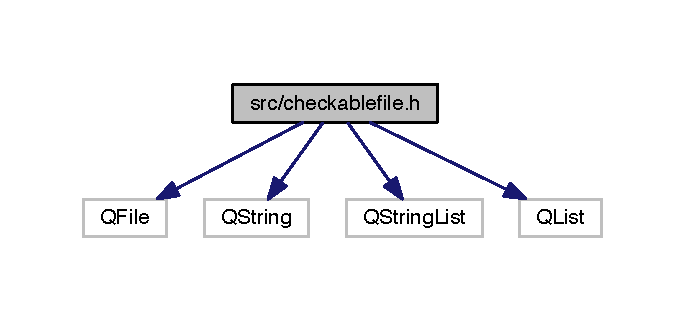
\includegraphics[width=329pt]{checkablefile_8h__incl}
\end{center}
\end{figure}
This graph shows which files directly or indirectly include this file\+:
\nopagebreak
\begin{figure}[H]
\begin{center}
\leavevmode
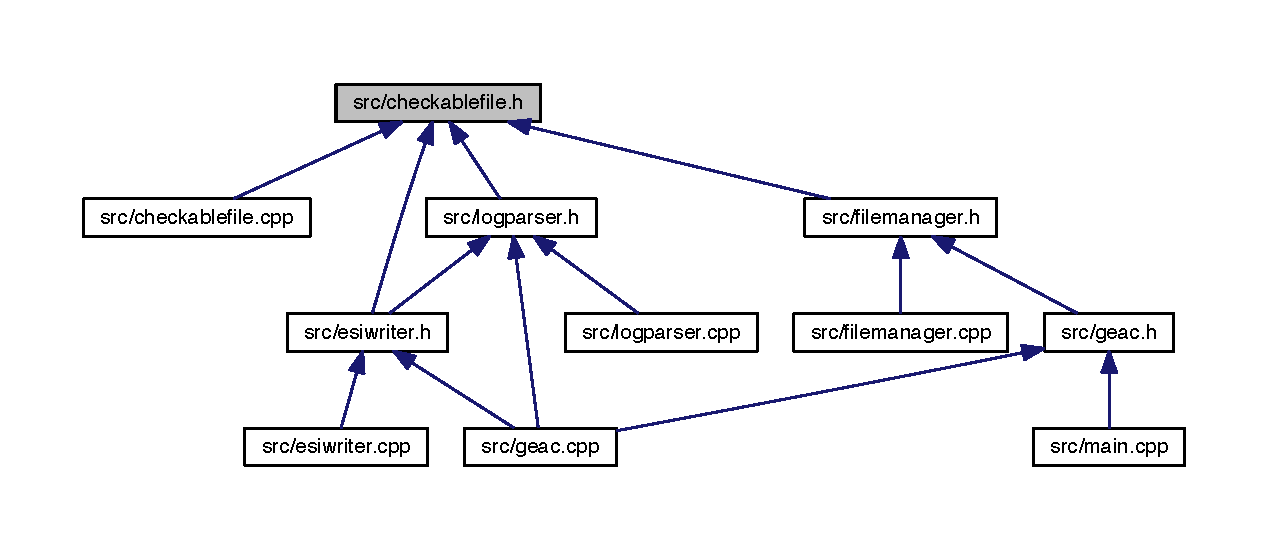
\includegraphics[width=350pt]{checkablefile_8h__dep__incl}
\end{center}
\end{figure}
\subsection*{Classes}
\begin{DoxyCompactItemize}
\item 
struct \hyperlink{struct_atom}{Atom}
\item 
class \hyperlink{class_checkable_file}{Checkable\+File}
\end{DoxyCompactItemize}

\hypertarget{checkfiledialog_8cpp}{}\section{src/checkfiledialog.cpp File Reference}
\label{checkfiledialog_8cpp}\index{src/checkfiledialog.\+cpp@{src/checkfiledialog.\+cpp}}
{\ttfamily \#include \char`\"{}checkfiledialog.\+h\char`\"{}}\\*
{\ttfamily \#include $<$Q\+H\+Box\+Layout$>$}\\*
{\ttfamily \#include $<$Q\+Dialog\+Button\+Box$>$}\\*
{\ttfamily \#include $<$assert.\+h$>$}\\*
Include dependency graph for checkfiledialog.\+cpp\+:
\nopagebreak
\begin{figure}[H]
\begin{center}
\leavevmode
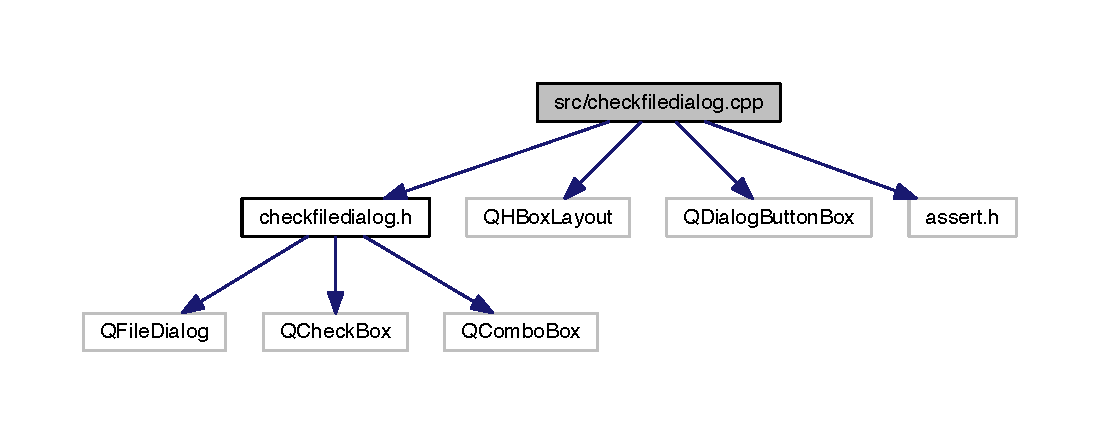
\includegraphics[width=350pt]{checkfiledialog_8cpp__incl}
\end{center}
\end{figure}

\hypertarget{checkfiledialog_8h}{}\section{src/checkfiledialog.h File Reference}
\label{checkfiledialog_8h}\index{src/checkfiledialog.\+h@{src/checkfiledialog.\+h}}
{\ttfamily \#include $<$Q\+File\+Dialog$>$}\\*
{\ttfamily \#include $<$Q\+Check\+Box$>$}\\*
{\ttfamily \#include $<$Q\+Combo\+Box$>$}\\*
Include dependency graph for checkfiledialog.\+h\+:
\nopagebreak
\begin{figure}[H]
\begin{center}
\leavevmode
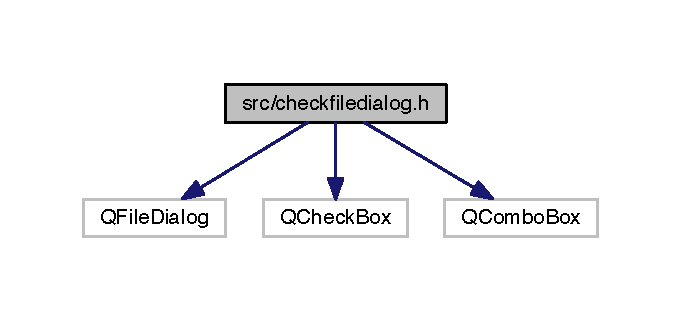
\includegraphics[width=327pt]{checkfiledialog_8h__incl}
\end{center}
\end{figure}
This graph shows which files directly or indirectly include this file\+:
\nopagebreak
\begin{figure}[H]
\begin{center}
\leavevmode
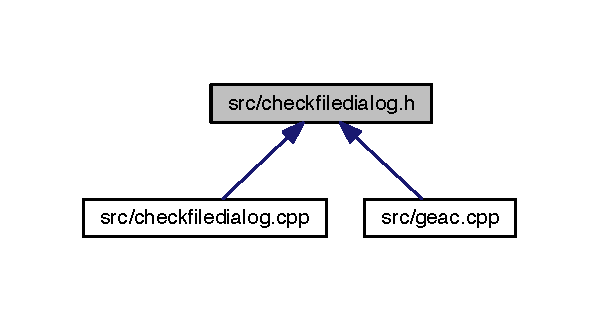
\includegraphics[width=288pt]{checkfiledialog_8h__dep__incl}
\end{center}
\end{figure}
\subsection*{Classes}
\begin{DoxyCompactItemize}
\item 
class \hyperlink{class_check_file_dialog}{Check\+File\+Dialog}
\end{DoxyCompactItemize}

\hypertarget{esiwriter_8cpp}{}\section{src/esiwriter.cpp File Reference}
\label{esiwriter_8cpp}\index{src/esiwriter.\+cpp@{src/esiwriter.\+cpp}}
{\ttfamily \#include \char`\"{}esiwriter.\+h\char`\"{}}\\*
{\ttfamily \#include $<$Q\+Message\+Box$>$}\\*
{\ttfamily \#include $<$Q\+Text\+Stream$>$}\\*

\hypertarget{esiwriter_8h}{}\section{src/esiwriter.h File Reference}
\label{esiwriter_8h}\index{src/esiwriter.\+h@{src/esiwriter.\+h}}
{\ttfamily \#include $<$Q\+Dir$>$}\\*
{\ttfamily \#include $<$Q\+File$>$}\\*
{\ttfamily \#include $<$Q\+String$>$}\\*
{\ttfamily \#include $<$Q\+String\+List$>$}\\*
{\ttfamily \#include \char`\"{}logparser.\+h\char`\"{}}\\*
{\ttfamily \#include \char`\"{}checkablefile.\+h\char`\"{}}\\*
Include dependency graph for esiwriter.\+h\+:
\nopagebreak
\begin{figure}[H]
\begin{center}
\leavevmode
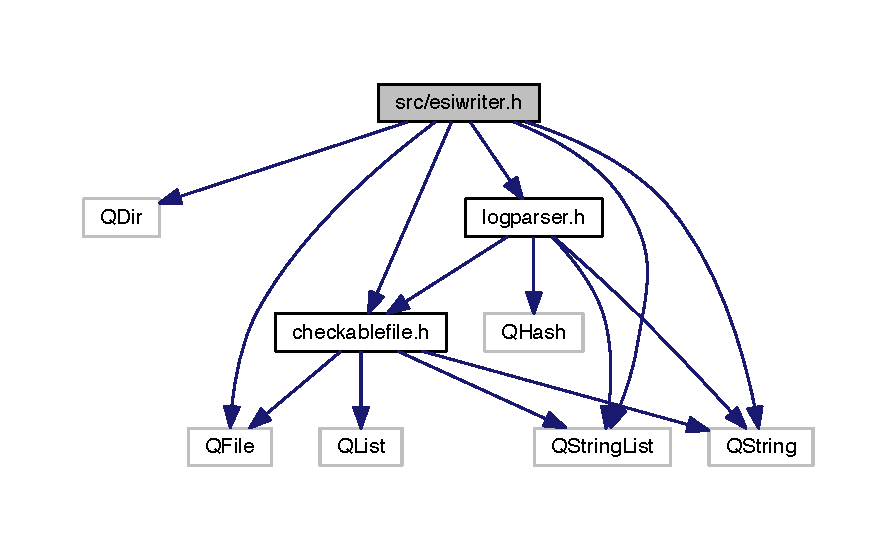
\includegraphics[width=350pt]{esiwriter_8h__incl}
\end{center}
\end{figure}
This graph shows which files directly or indirectly include this file\+:
\nopagebreak
\begin{figure}[H]
\begin{center}
\leavevmode
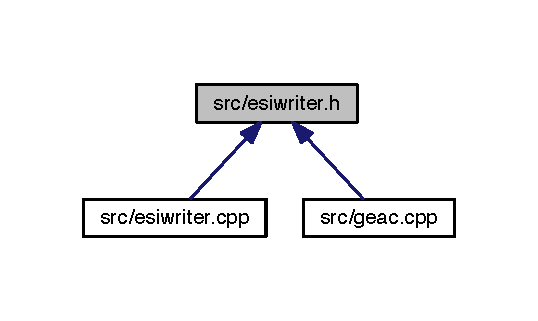
\includegraphics[width=258pt]{esiwriter_8h__dep__incl}
\end{center}
\end{figure}
\subsection*{Classes}
\begin{DoxyCompactItemize}
\item 
class \hyperlink{class_esi_writer}{Esi\+Writer}
\end{DoxyCompactItemize}

\hypertarget{filemanager_8cpp}{}\section{src/filemanager.cpp File Reference}
\label{filemanager_8cpp}\index{src/filemanager.\+cpp@{src/filemanager.\+cpp}}
{\ttfamily \#include \char`\"{}filemanager.\+h\char`\"{}}\\*
{\ttfamily \#include $<$Q\+Dir$>$}\\*

\hypertarget{filemanager_8h}{}\section{src/filemanager.h File Reference}
\label{filemanager_8h}\index{src/filemanager.\+h@{src/filemanager.\+h}}
{\ttfamily \#include $<$Q\+Abstract\+Table\+Model$>$}\\*
{\ttfamily \#include $<$Q\+Variant$>$}\\*
{\ttfamily \#include $<$Q\+List$>$}\\*
{\ttfamily \#include $<$Q\+String\+List$>$}\\*
{\ttfamily \#include \char`\"{}checkablefile.\+h\char`\"{}}\\*
\subsection*{Classes}
\begin{DoxyCompactItemize}
\item 
class \hyperlink{class_file_manager}{File\+Manager}
\end{DoxyCompactItemize}

\hypertarget{filemanagerdelegate_8cpp}{}\section{src/filemanagerdelegate.cpp File Reference}
\label{filemanagerdelegate_8cpp}\index{src/filemanagerdelegate.\+cpp@{src/filemanagerdelegate.\+cpp}}
{\ttfamily \#include \char`\"{}filemanagerdelegate.\+h\char`\"{}}\\*
{\ttfamily \#include $<$Q\+Painter$>$}\\*
{\ttfamily \#include $<$Q\+Text\+Option$>$}\\*
{\ttfamily \#include $<$Q\+Color$>$}\\*
{\ttfamily \#include $<$Q\+Svg\+Renderer$>$}\\*

\hypertarget{filemanagerdelegate_8h}{}\section{src/filemanagerdelegate.h File Reference}
\label{filemanagerdelegate_8h}\index{src/filemanagerdelegate.\+h@{src/filemanagerdelegate.\+h}}
{\ttfamily \#include $<$Q\+Styled\+Item\+Delegate$>$}\\*
{\ttfamily \#include $<$Q\+Size$>$}\\*
\subsection*{Classes}
\begin{DoxyCompactItemize}
\item 
class \hyperlink{class_file_manager_delegate}{File\+Manager\+Delegate}
\end{DoxyCompactItemize}

\hypertarget{geac_8cpp}{}\section{src/geac.cpp File Reference}
\label{geac_8cpp}\index{src/geac.\+cpp@{src/geac.\+cpp}}
{\ttfamily \#include \char`\"{}geac.\+h\char`\"{}}\\*
{\ttfamily \#include $<$Q\+File\+Dialog$>$}\\*
{\ttfamily \#include $<$Q\+Settings$>$}\\*
{\ttfamily \#include $<$Q\+Future$>$}\\*
{\ttfamily \#include $<$Qt\+Concurrent$>$}\\*
{\ttfamily \#include \char`\"{}checkfiledialog.\+h\char`\"{}}\\*
{\ttfamily \#include \char`\"{}logparser.\+h\char`\"{}}\\*
{\ttfamily \#include \char`\"{}esiwriter.\+h\char`\"{}}\\*
Include dependency graph for geac.\+cpp\+:
\nopagebreak
\begin{figure}[H]
\begin{center}
\leavevmode
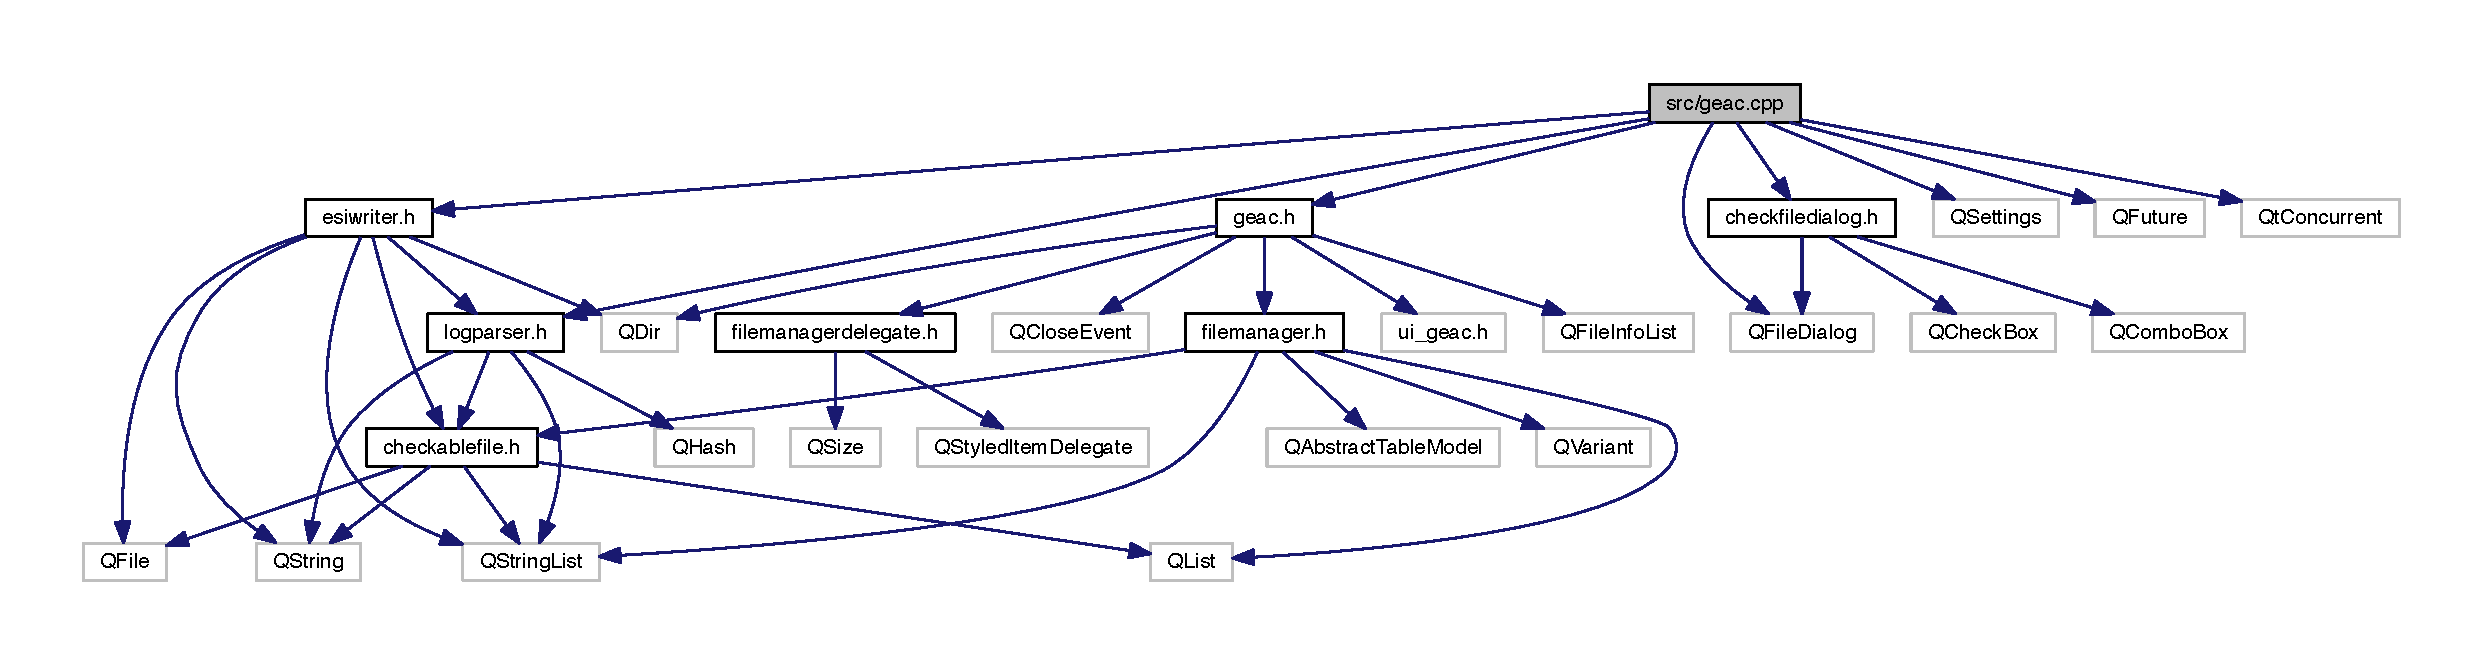
\includegraphics[width=350pt]{geac_8cpp__incl}
\end{center}
\end{figure}

\hypertarget{geac_8h}{}\section{src/geac.h File Reference}
\label{geac_8h}\index{src/geac.\+h@{src/geac.\+h}}
{\ttfamily \#include \char`\"{}ui\+\_\+geac.\+h\char`\"{}}\\*
{\ttfamily \#include $<$Q\+Dir$>$}\\*
{\ttfamily \#include $<$Q\+File\+Info\+List$>$}\\*
{\ttfamily \#include $<$Q\+Close\+Event$>$}\\*
{\ttfamily \#include \char`\"{}filemanager.\+h\char`\"{}}\\*
{\ttfamily \#include \char`\"{}filemanagerdelegate.\+h\char`\"{}}\\*
\subsection*{Classes}
\begin{DoxyCompactItemize}
\item 
class \hyperlink{class_geac}{Geac}
\end{DoxyCompactItemize}

\hypertarget{logparser_8cpp}{}\section{src/logparser.cpp File Reference}
\label{logparser_8cpp}\index{src/logparser.\+cpp@{src/logparser.\+cpp}}
{\ttfamily \#include \char`\"{}logparser.\+h\char`\"{}}\\*
{\ttfamily \#include $<$Q\+Regular\+Expression$>$}\\*
{\ttfamily \#include $<$Q\+Regular\+Expression\+Match$>$}\\*
{\ttfamily \#include $<$Q\+Debug$>$}\\*
Include dependency graph for logparser.\+cpp\+:
\nopagebreak
\begin{figure}[H]
\begin{center}
\leavevmode
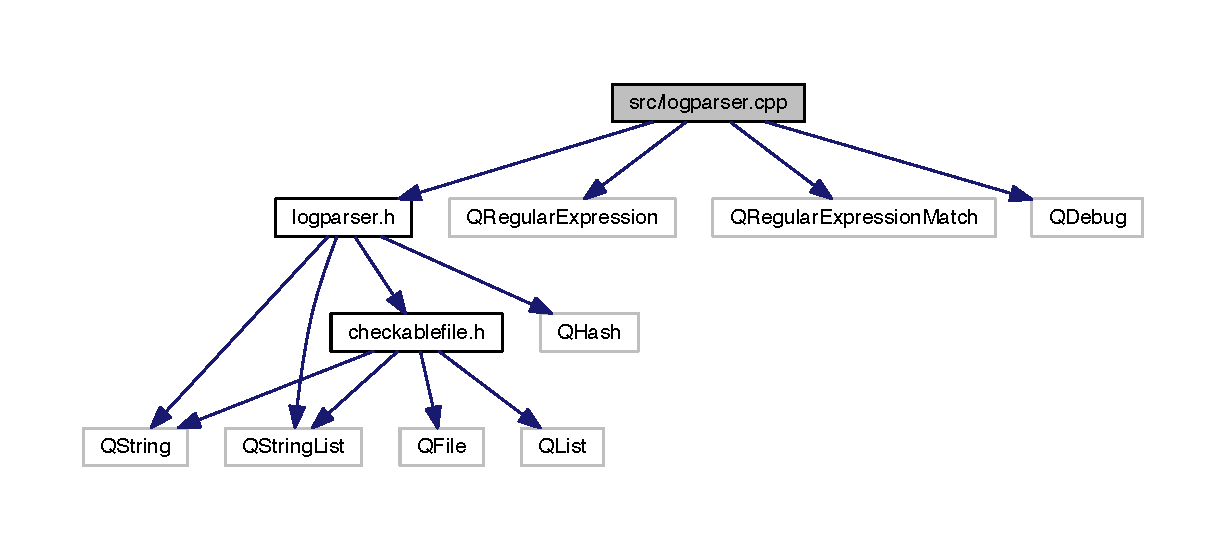
\includegraphics[width=350pt]{logparser_8cpp__incl}
\end{center}
\end{figure}

\hypertarget{logparser_8h}{}\section{src/logparser.h File Reference}
\label{logparser_8h}\index{src/logparser.\+h@{src/logparser.\+h}}
{\ttfamily \#include $<$Q\+String$>$}\\*
{\ttfamily \#include $<$Q\+String\+List$>$}\\*
{\ttfamily \#include $<$Q\+Hash$>$}\\*
{\ttfamily \#include \char`\"{}checkablefile.\+h\char`\"{}}\\*
\subsection*{Classes}
\begin{DoxyCompactItemize}
\item 
class \hyperlink{class_log_parser}{Log\+Parser}
\end{DoxyCompactItemize}

\hypertarget{main_8cpp}{}\section{src/main.cpp File Reference}
\label{main_8cpp}\index{src/main.\+cpp@{src/main.\+cpp}}
{\ttfamily \#include $<$Q\+Application$>$}\\*
{\ttfamily \#include $<$Q\+Translator$>$}\\*
{\ttfamily \#include $<$Q\+Library\+Info$>$}\\*
{\ttfamily \#include \char`\"{}geac.\+h\char`\"{}}\\*
\subsection*{Functions}
\begin{DoxyCompactItemize}
\item 
int \hyperlink{main_8cpp_a0ddf1224851353fc92bfbff6f499fa97}{main} (int argc, char $\ast$argv\mbox{[}$\,$\mbox{]})
\end{DoxyCompactItemize}


\subsection{Function Documentation}
\hypertarget{main_8cpp_a0ddf1224851353fc92bfbff6f499fa97}{}\index{main.\+cpp@{main.\+cpp}!main@{main}}
\index{main@{main}!main.\+cpp@{main.\+cpp}}
\subsubsection[{main}]{\setlength{\rightskip}{0pt plus 5cm}int main (
\begin{DoxyParamCaption}
\item[{int}]{argc, }
\item[{char $\ast$}]{argv\mbox{[}$\,$\mbox{]}}
\end{DoxyParamCaption}
)}\label{main_8cpp_a0ddf1224851353fc92bfbff6f499fa97}

%--- End generated contents ---

% Index
\backmatter
\newpage
\phantomsection
\clearemptydoublepage
\addcontentsline{toc}{chapter}{Index}
\printindex

\end{document}
